\chapter{Design and Development of the
Proposed Solution
}

\renewcommand{\chaptername}{Chapter}
\section*{Introduction}

This chapter details the design and development of the proposed path planning solution for logistics forklifts. 
The focus is on linking the robot to a pallet in the tight stations of a warehouse as a last maneuver to the 
pickup/drop process. The system uses pattern-based paths, elevated by meta-heuristic algorithms, to navigate 
efficiently in these confined areas. 
The chapter begins with 
an overview of the goals and the work structure, followed by an outline of the development steps used to ensure 
smooth and accurate movement toward the pallet. Implementation details are then covered, showing how the system 
components are integrated into a cohesive solution for precise pallet access within the warehouse environment.

\section{Conceptual Framework}
\subsection{Goal Setting}
%goals and overall approach of the methodology
As mentioned in the introduction, this project does not tackle the navigation system of the AMRs in 
general, but is focusing on a specific movement that the AMR must perform in order to accurately dock the pallet/shelf. 
More details are explained in chapter 1, section 2.
Considered the problems detailed in chapter 1 and the state of the art outputs in chapter 2, 
the following goals were identified 
based on the former detailed requirements for applications to autonomous mobile robots in intralogistics:
\begin{itemize}
    \item \textbf{Predictability and Robustness of Mobile Robot Behavior: }The solution we propose utilizes an intelligent approach to connect 
    the robot to its destination. The developed algorithm generates an explainable navigation process that enables humans 
    to understand and trust the technology. Additionally, secure decision-making for autonomous trucks is ensured by the 
    developers. 

    \item \textbf{Accuracy of the solution and station relation: }The developed solution has to be stable, repeatable and flexible: this 
    means that it would work for almost all stations in warehouses where it operates. The linking to the destination is 
    accurate and precise to avoid failures. Precision and accuracy are guaranteed by the fact that the planning is done 
    in the limited station space: a narrow field that allows short distance perception and planning. The solution is 
    then tailored to each environment's specificities. 
    
    \item \textbf{Optimization of paths: }The algorithm optimizes the path by minimizing travel distance, reducing sudden turns, and avoiding challenging maneuvers that could 
    strain the truck. This optimization ensures the most efficient route, balancing speed and safety. The approach is designed to be 
    computationally efficient, allowing for real-time adjustments and smooth behavior of the autonomous truck.

    \item \textbf{Obstacle avoidance: }The vehicle avoids collisions and drives safely to its destination. The system is designed to 
    prioritize safety while maintaining an efficient and effective route to the target location.

\end{itemize}


\subsection{Development Methodology} %TODO: hedhi design
To achieve the aforementioned goals, the design  will follow a structured approach, consisting of the following key 
development steps: 

\begin{itemize}
    \item Station Layout Analysis: An analysis of the station layout enhances the development 
    of station-specific solution. The analysis considers the differences in the stations dimensions
    and configurations and the solution is created in station relation to ensure precision and accuracy
    to potential changes like shelf shifts and unkown obstacles (obstacles that do not initially 
    belong to the station). Understanding station layouts can improve path optimization, reduce the need for 
    frequent replanning, and enhance the overall efficiency of operations.

    \item Path Generation: A robust and efficient path generation algorithm is developed and tailored to 
    the station environment. The path follows human-driving patterns along with specific rules and constraints 
    which enhances efficiency, predictability and makes use of explainable AI concepts.

    \item Path Optimization: Metaheuristic Algorithms are tested in different station configuration scenarios 
    and discriminated. The most suitable algorithm in terms of processing time is considered. The optimizer 
    generates an optimum path for specific criteria. 

    \item Obstacle Avoidance: obstacles are avoided using the pattern path and optimizer constraints.

\end{itemize}

To overcome the drawbacks of the methods in Chapter 2, Our approach focuses on:
\begin{itemize}
    \item Repeatability: by generating pattern based paths, the AMR's behavior is explainable at 
    the linking phase: the AMR uses the pattern to create optimized trajectories and takes into 
    consideration the environmental input. The simplicity of the approach makes it require a minimum 
    amount of information and computational power. 
    \item Operational Reliability: Tailoring the solution to the station and acquiring real-time sensor data about
    the target's location guarantees accurate path generation, as the generation of the path is processed 
    according to real-world data instead of model data. 
    This approach enhances task success rates and reduces path length due to the confined station environment.

    \item Computational Optimization: The approach uses Metaheuristic Optimization approaches
    to refine and discriminate already created paths using the pattern instead of building the path 
    from scratch using 
    the optimizer. This significantly improves computational efficiency. 

    \item Kinematic constraints: The approach takes into consideration the volume of the truck and its 
    constraints like reduced speed at highly curved areas and when direction changes are needed. 
    The pattern-based approach further restricts directional changes, ensuring adherence to kinematic 
    constraints and optimizing path generation.
\end{itemize}

The following sections will detail the design  approach. Then, the implementation steps are 
explicited and demonstrated from the simulation point of view. Finally, the tests results are explained 
and discussed and the outlooks are elaborated. 

\section{Methodology and Design of the Solution}

Starting with the operating environment, the stations, the focus was on the problems inside. The issue of linking 
the forklifts in the near-field to the pallet is nothing but new to the intralogistics sector. 
The process is repeated dozens of times daily inside warehouses and factories where forklift drivers take control over 
resolving the problem. Taking a deeper look at their approaches to resolve the same issue, the autonomous vehicles team 
noticed that forklift drivers have certain driving styles that are repeated according to the current situation.
Similarily to car parking, depending on the type of the parking slot, there are some patterns to reproduce in order to fit 
the car inside its assigned spot as given by figure \ref{Parking_Styles}. 
Each situation has an according pattern that is relevant to the car's orientation, the parking slot, 
and the direction of parking. The parking styles were set to teach beginners the way to park a car 
smoothly: stopping and changing directions are minimized by the shape of the path.
The path is smooth and designed in a way to make steering possible online for instance in angle 
amd perpendicular parking. For, Parallel and Perpendicular Back Parking, direction changes 
are needed to  put the vehicle in a position where it can smoothly steer and rejoin the parking slot.
The Perpendicular Back Parking is very similar to the forklift in the station case.
The car arrives in main driving direction but needs to dock the slot in a backward direction. 
The parking pattern has 2 maneuvers: a first maneuver of direction change and a second maneuver of 
placing the carf inside its slot.
In these cases, the driver needs 
enough space for direction changing. To do so, he drives further to the opposite direction to allow 
the car to comfortably and smoothly drive to its parking place while steering gradually to correct the orientation.
Parking assistance feature is embedded in human-driven and driverless cars to instill safety and order.

\begin{figure}
    [H]
    \begin{center}
    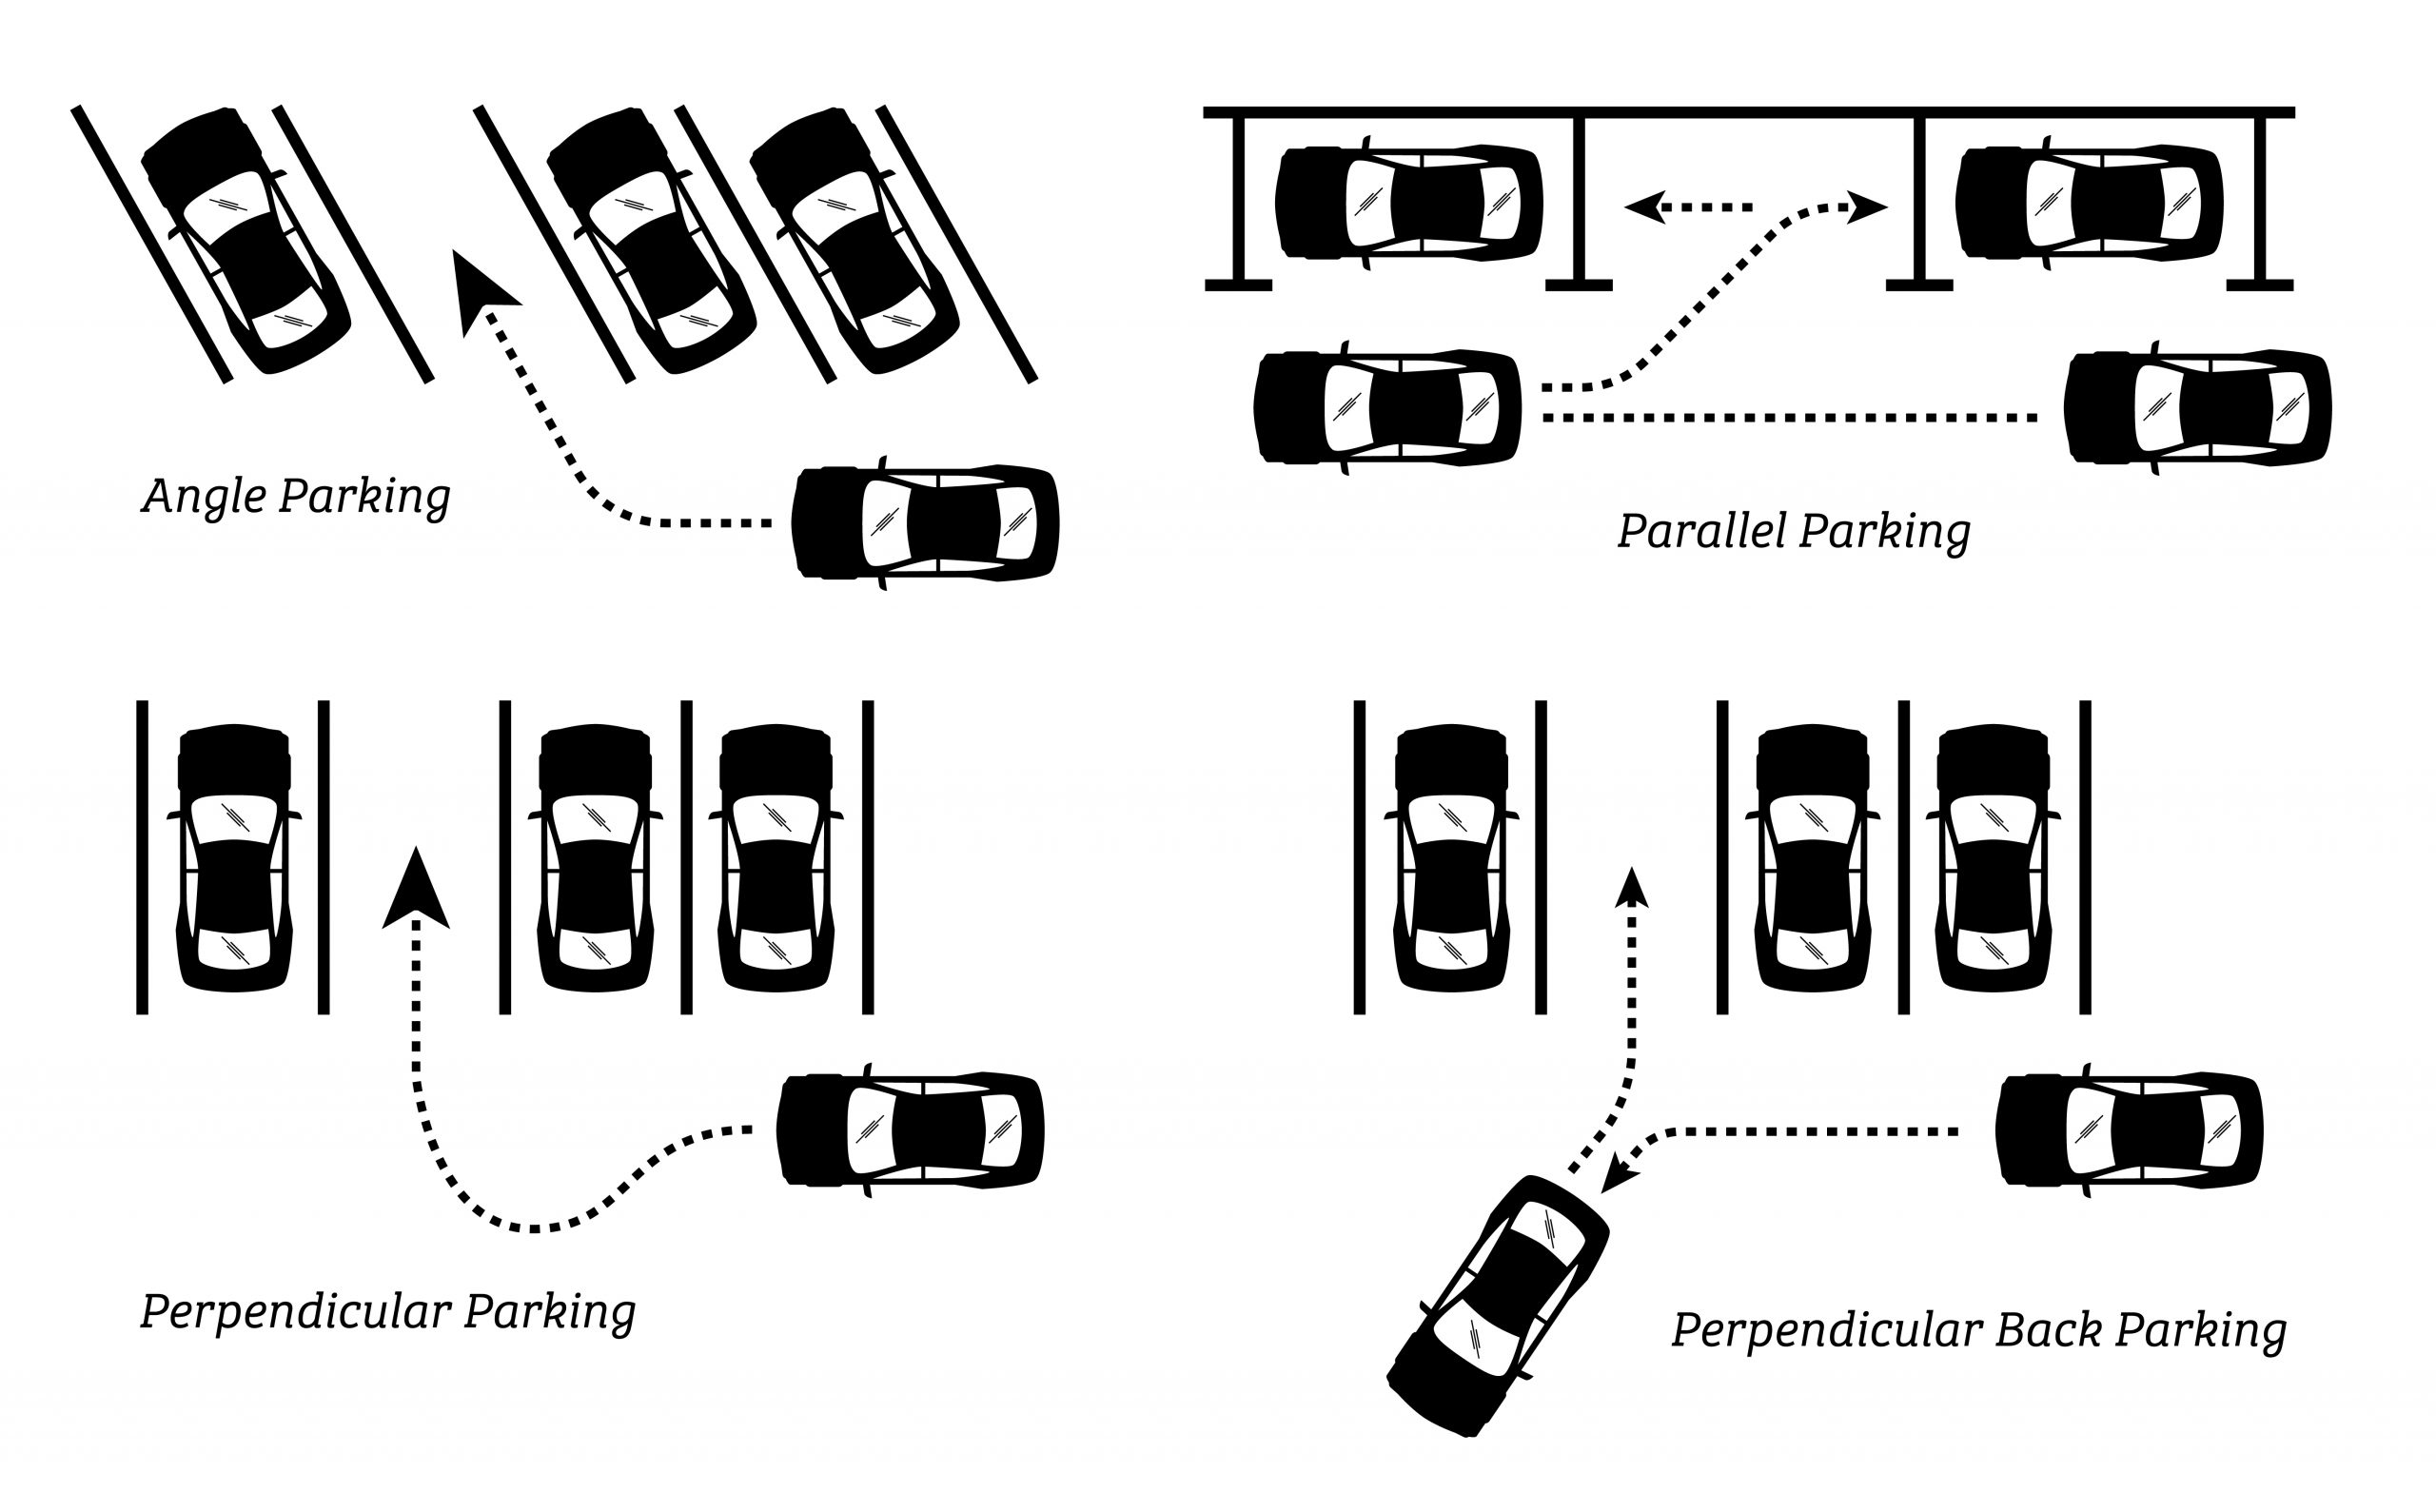
\includegraphics[width=4in]{images/Chap2/perpendicular-parking-a-lot-scaled.jpg}\\
    \caption{The Possible Parking Styles that a driver can follow}
    \label{Parking_Styles}
    \end{center}
\end{figure}

Analogically, after the truck arrives in the station, the drivers would drive and steer in the opposite direction of the 
pallet, until the forks are in a position to allow the truck to easily and correctfully drive to the pallet in fork direction.
The goal here is to develop a pallet-linking algorithm to automate the driving to the pallet pickup location for 
autonomous forklifts as given by figure \ref{pattern}. The truck would autonomously plan the path to its destination
based on the pattern: the Station linking trajectory on figure \ref{pattern} and on the environment settings that it would navigate in. 
The pattern enhances the explainability in the forklifts behavior. Explainability allows for more order in the warehouse: 
it simplifies the coordination of safe simultaneous tasks around the truck. This is achieved through the design of an 
algorithm that aims to create a transparent navigation process, making it easier for humans to understand and trust 
the technology. Additionally, the approach is intended to ensure secure and reliable decision-making for autonomous trucks.



\begin{figure}
    [H]
    \begin{center}
    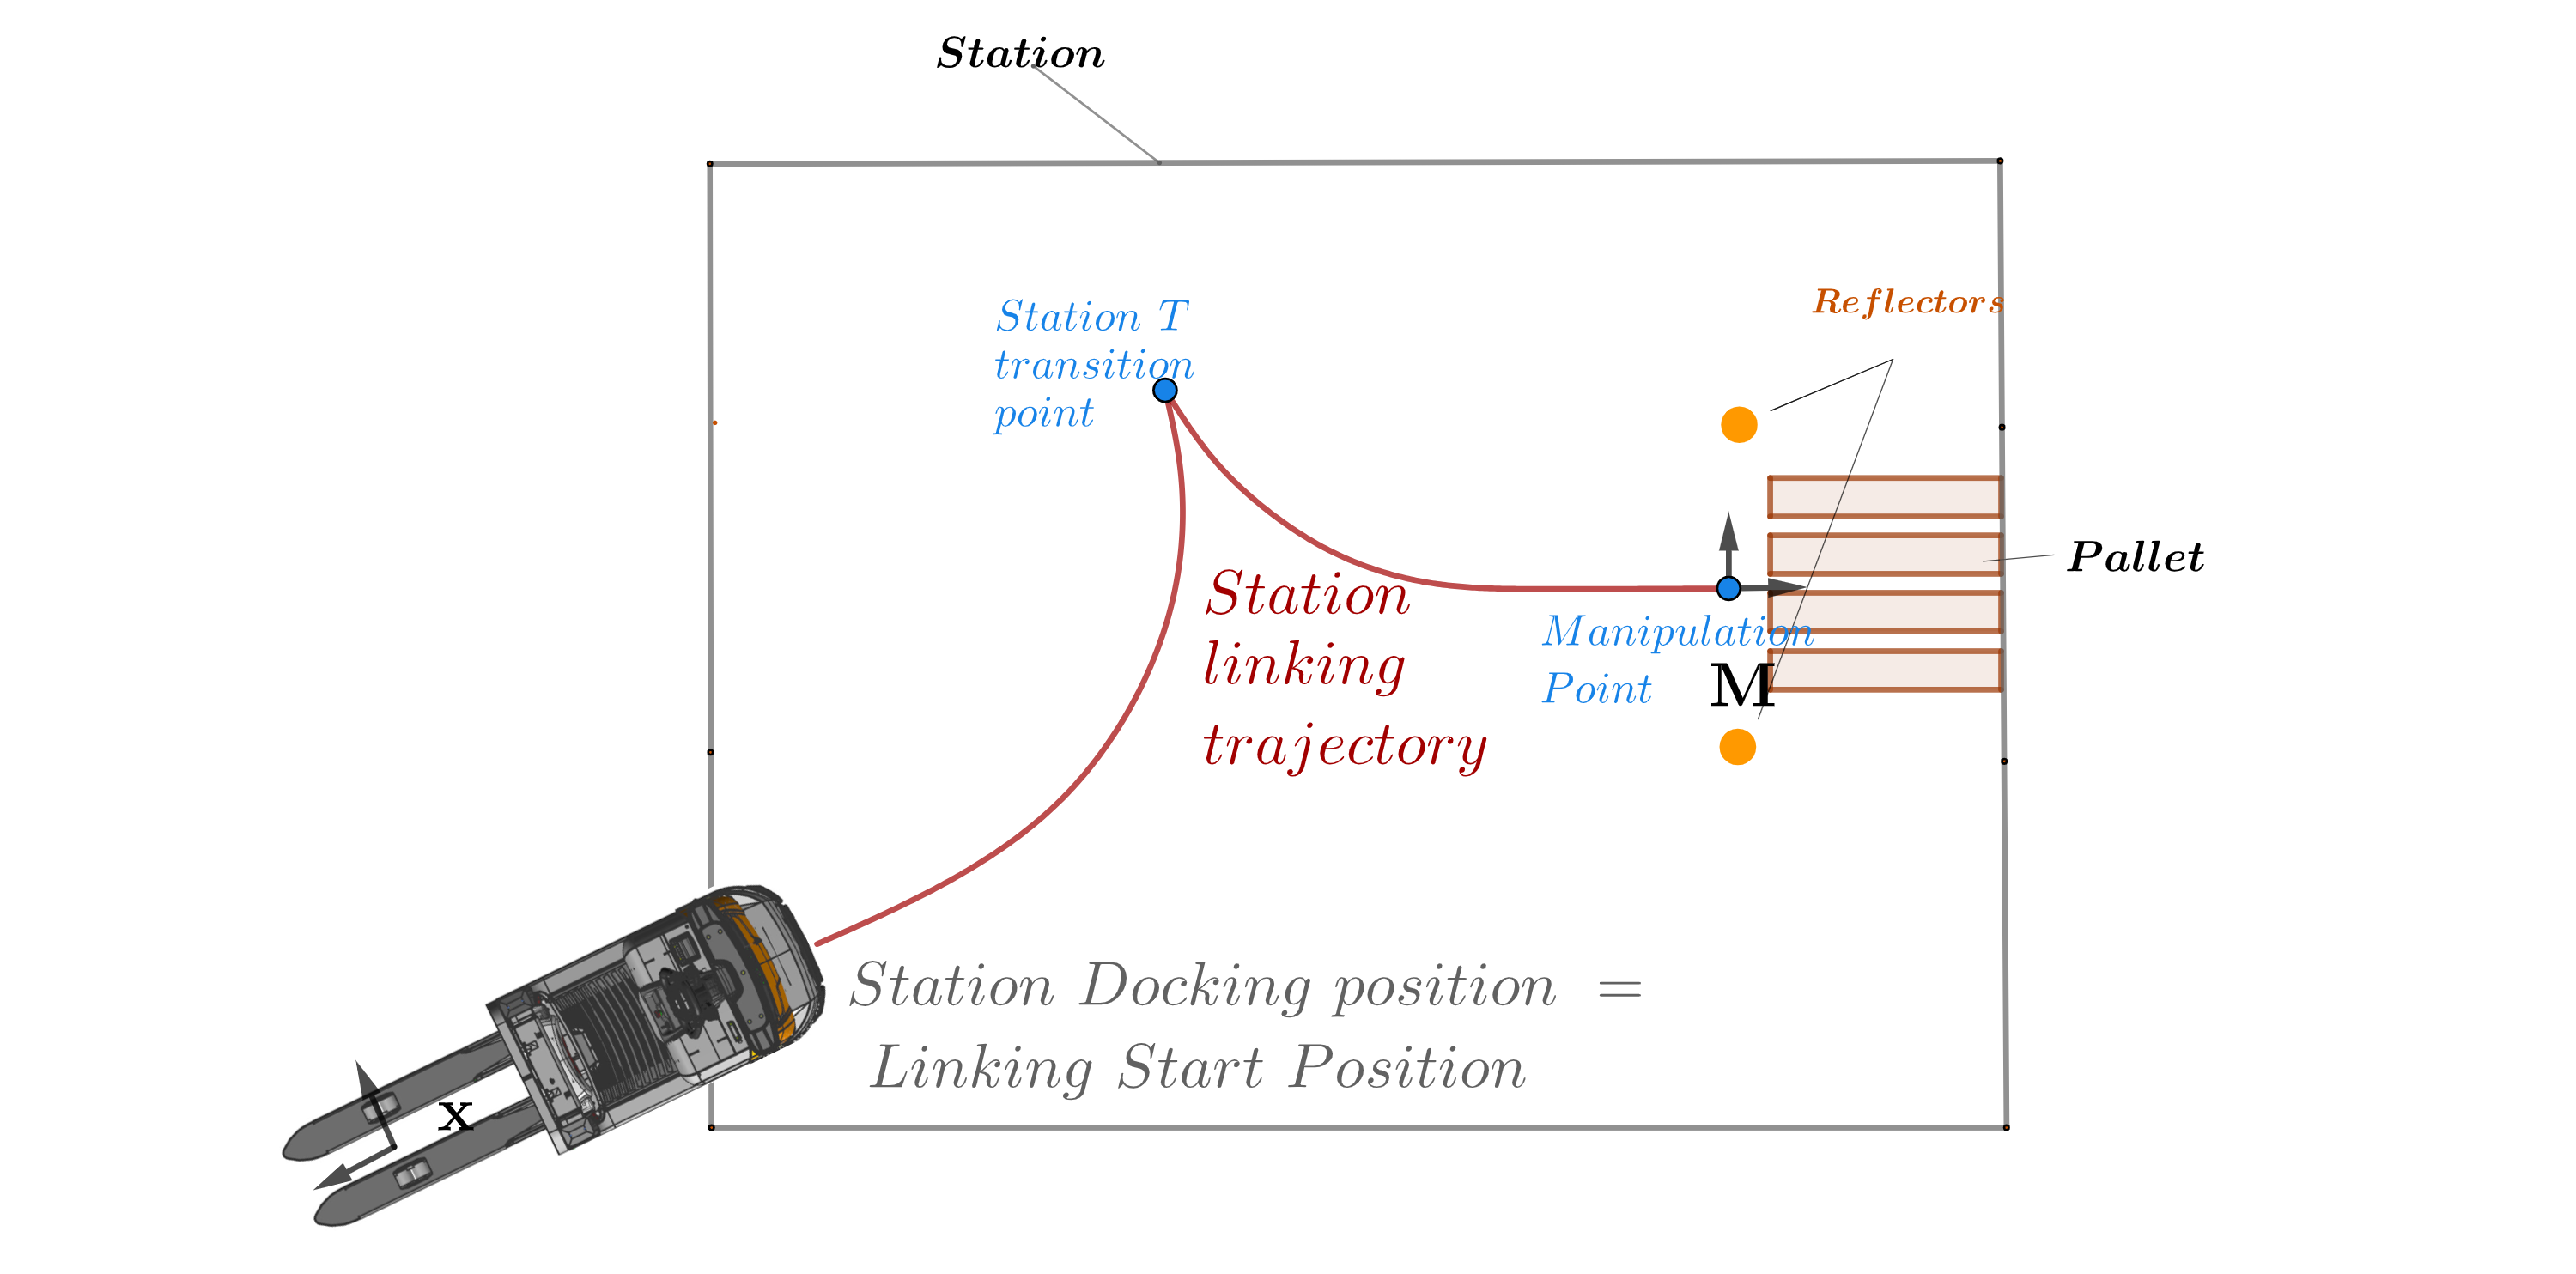
\includegraphics[width=\linewidth]{images/Chap2/station-without-subpolygones.png}\\
    \caption{Design of Linking the robot to goal destination \cite{R28}}
    \label{pattern}
    \end{center}
\end{figure}
For the forklifts use case, the AMR enters the station in "Opposite Direction" and docks the shelf/pallet in 
"Main Direction" simliarily to the Back Perpendicular Parking.
From now on, the following definitions of driving directions will be used as gven by figure \ref{driving directions}:
\begin{itemize}
    \item Main Driving Direction: Driving in fork direction.
    \item Opposite Driving Direction: Driving in vehicle chassis direction.
\end{itemize}

\begin{figure}
    [!ht]
    \begin{center}
    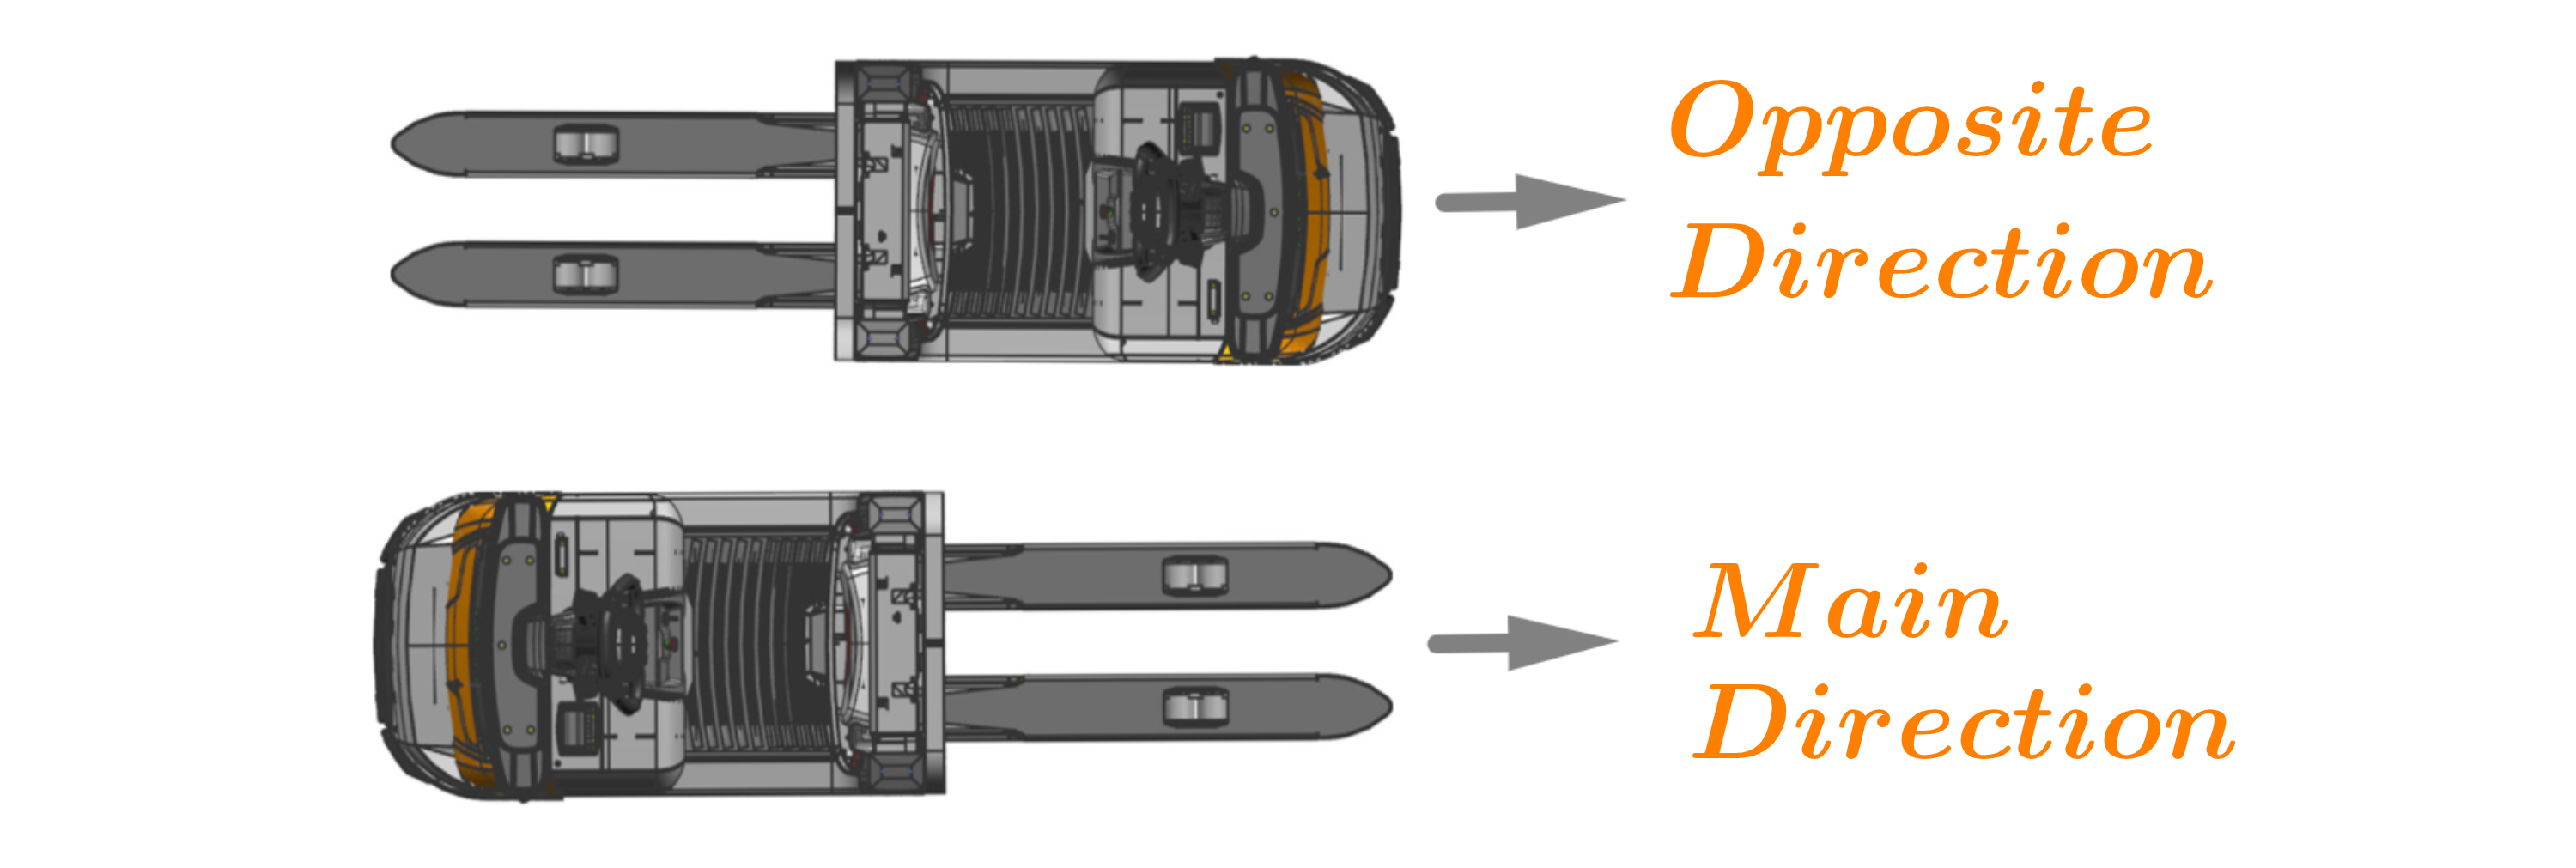
\includegraphics[width=4in]{images/Chap2/driving_directions.png}\\
    \caption{Truck Driving Directions}
    \label{driving directions}
    \end{center}
\end{figure} 
 
The designed approach is illustrated in figure \Ref{design}.
The following transition method is prposed: 
Once the AMR docks the station, it has the option to transition and change 
direction on the sides of the shelf placed inside the station. First, it drives to the transition position, then, to the 
pallet or the drop-off position as given by figure \Ref{subpolygons}. Having two possibilities for transition zones allows 
for more flexibility: 
in case one area is unreachable or presents obstacles, the second one can be used. They present free areas 
inside the stations where less obstacles and dynamics are expected and smooth maneuvering of the truck can be managed. 
In addition, the geometric solution is scalable to 
any station that is recognized and whose properties are available to the truck. This makes the overall solution and the 
autonomous forklifts simple to
commission in new warehouses.

\begin{figure}
    [!ht]
    \begin{center}
    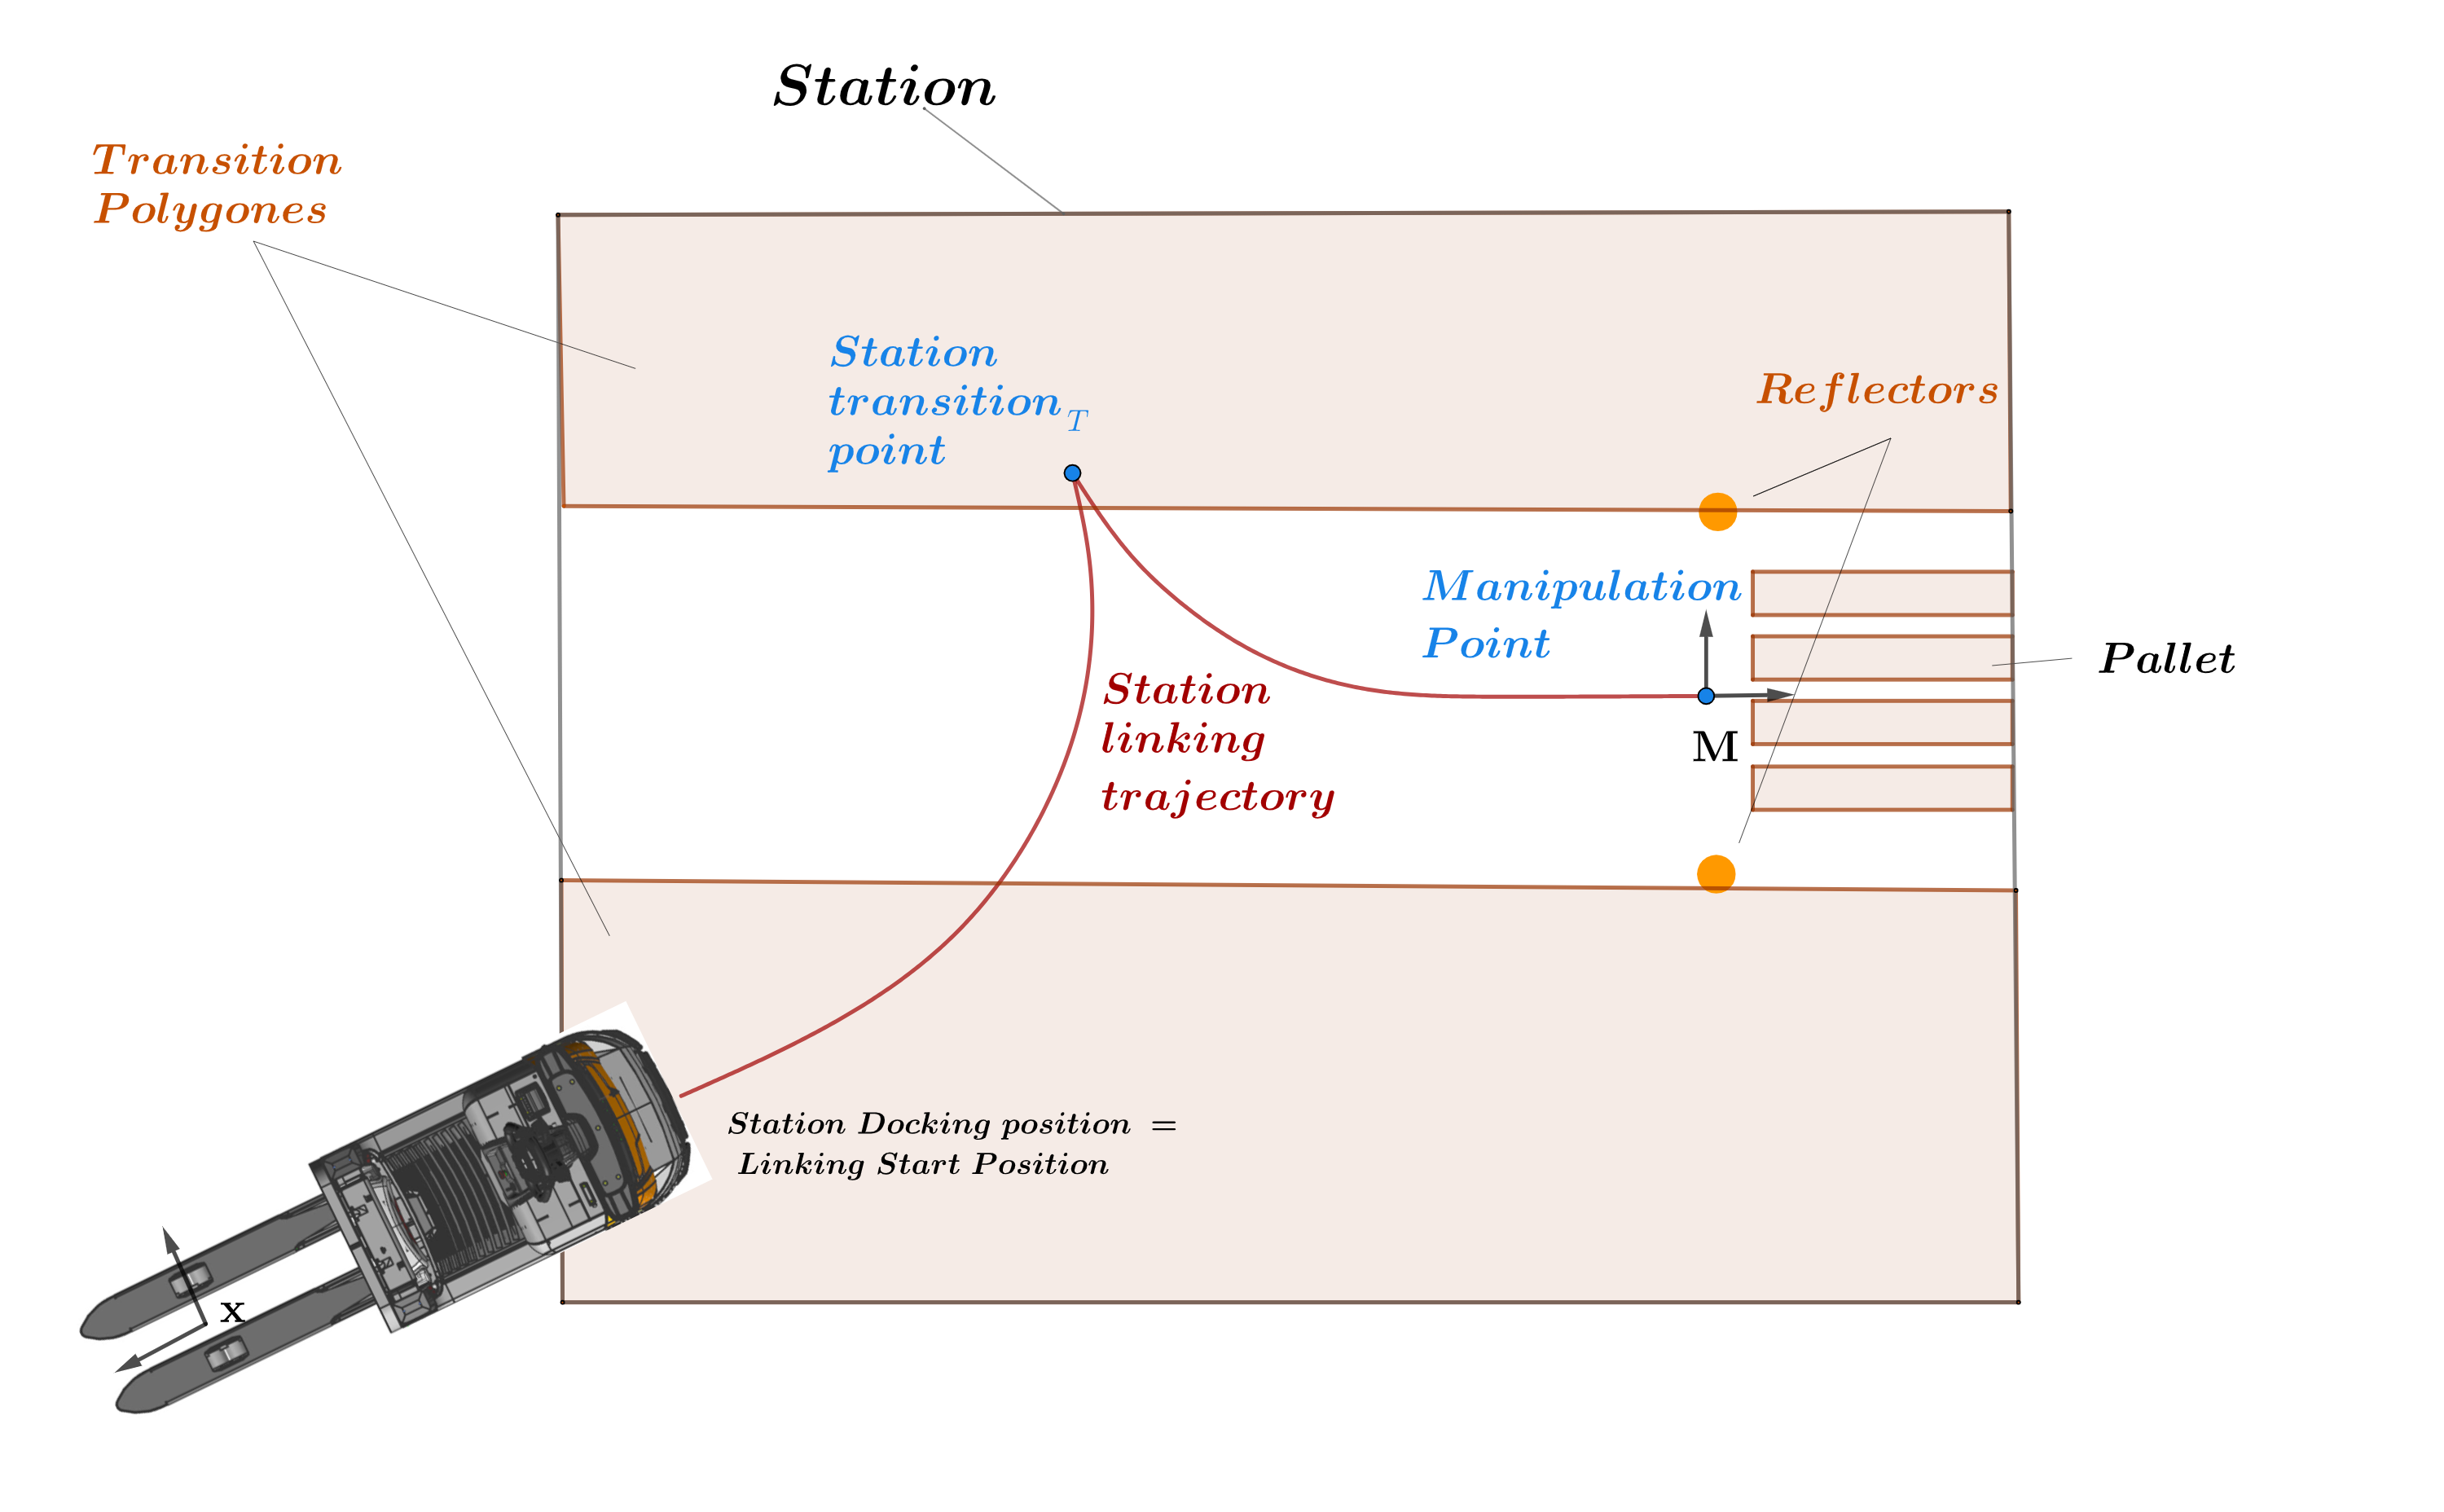
\includegraphics[width=\linewidth]{images/Chap2/station-without-subpolygones (2).png}\\
    \caption{Step1: Station Partitioning for Linking the robot to goal pallet \cite{R28}}
    \label{subpolygons}
    \end{center}
\end{figure}

Smooth and continuous paths are generated through spline interpolation of constructed waypoints (see section 3.2.2). 
This technique ensures 
that the resulting paths are smooth, operationally seamless, and reduce abrupt changes in direction and speed. 
By interpolating between waypoints, the method enables the creation of curves that are optimized for driving efficiency 
and stability.

Finally, an optimizer  
generates multiple path candidates and rigorously evaluates each one based on key factors. 
The evaluation considers the path's length, smoothness, and potential collisions with surrounding objects to ensure the 
chosen path is both efficient and safe. After testing all options, the path that best meets these 
criteria—providing the shortest and smoothest route with minimal collision risk—is selected as the best solution
following Evaluation methods expalined more in section 3.3. 

This approach ensures the final path is not only theoretically ideal but also practical and reliable for real-world use. 
The process is designed to be flexible and effective, even in obstacle environments. The designed methodology 
is summarized in the following flowchart \ref{design}:

\begin{figure}[H]
    \begin{center}
        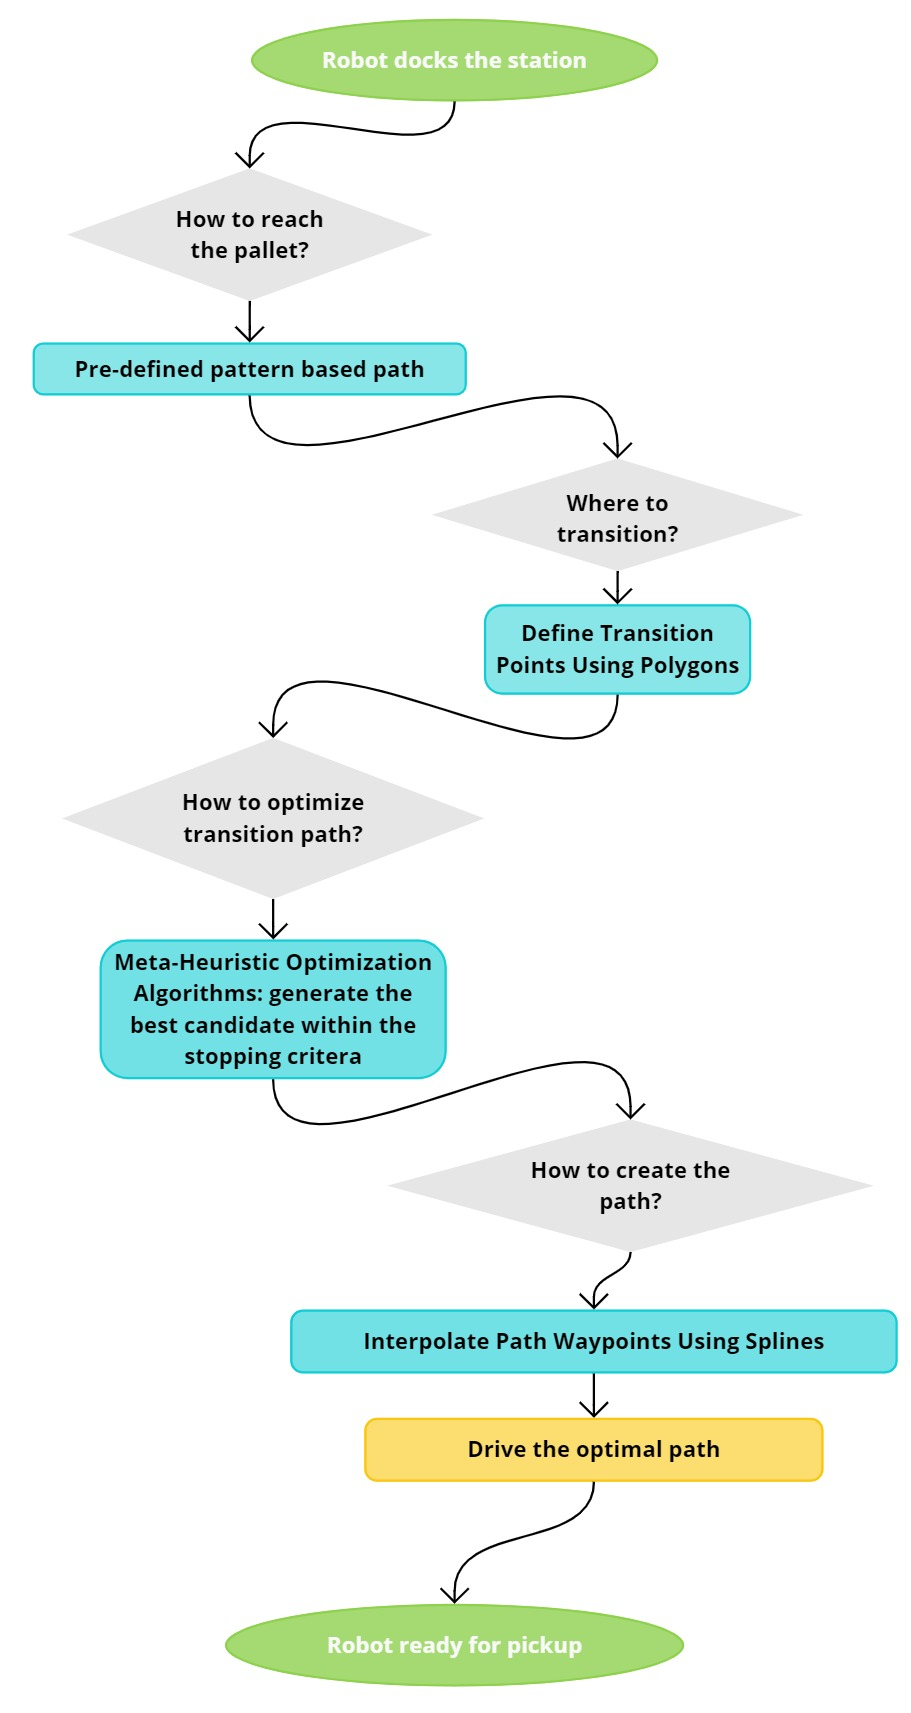
\includegraphics[width=4in]{images/Chap2/Approch_design.jpg}\\
        \caption{Milestones of the Path planning approach to pallet docking}
        \label{design}
        \end{center}
\end{figure}

\section{Development phases and Implementation}

This section details the rollout of the module development, providing a comprehensive overview of the process. 
It is structured to include both the development steps and the corresponding simulation results at each phase.
Every phase started with a deep investigation of the existing relevant solutions detailed in Chapter 2.

\subsection{Geometric Partitioning of the Station}
This section explains the development of the geometric Partitioning of the station into 2 polygons used later for 
transitioning inside the station. \textbf{The input of this step is the station information and the output are the polygons}.
As explained previously in Section 3.2, in order to carry out the transitioning of the vehicle inside 
the station to change the driving direction from the opposite to the main direction, Transition subpolygons are needed. 
The subpolygons are created according to the station shape and dimensions and the position of the shelf inside of it. 
As given by figure \ref{warehouse}, the stations can be found at certain positions of the warehouse.

\subsubsection{Implementation of the Station Partitioning}
The vehicle initially plans its missions: it constructs a plan of the stations that will be visited and the operations
to do on each station. While the path driven from one station to the other is pre-defined by the global planner, 
the path linking the vehicle to the pallet is to be planned in real-time. 
Once the vehicle arrives at the docking position in the stations, it starts the path planning process. 
The station-related information are stored in a file accessible to the vehicle. These information include stations' 
positions and dimensions and the coordinates of the shelf that it contains.
For each station represented like figure \ref{Station} the module creates the subpolygons on each side of the shelf, 
limited by the station and shelf shapes. 

The process that creates the subpolygons is detailed in the following Algorithm \ref{alg:createSubpolygons}.
The algorithm begins with an initialization step, then the corners of the station and shelf areas are retrieved and 
transformation matrices are prepared to convert coordinates between global and shelf-specific coordinate systems. 
The need to transform the used coordinates to the shelf frame is derived from the scalability needs.
As seen on figure \Ref{warehouse}, stations can be placed in different positions and have different orientations.
If global coordinates are used, it becomes computationally challenging to develop an exhaustive algorithm that fits all the 
possibilities of station orientation and shelf configurations. On the other hand, using the shelf coordinate frame shifts 
the point of view to the inside of the station only. It enables the shelf to orchestrate the geometric partitioning 
of the station based on its position in the station.

The transformation matrix from the shelf to Global is illustrated in figure \Ref{Station}.

\begin{figure}[H]
    \begin{center}
        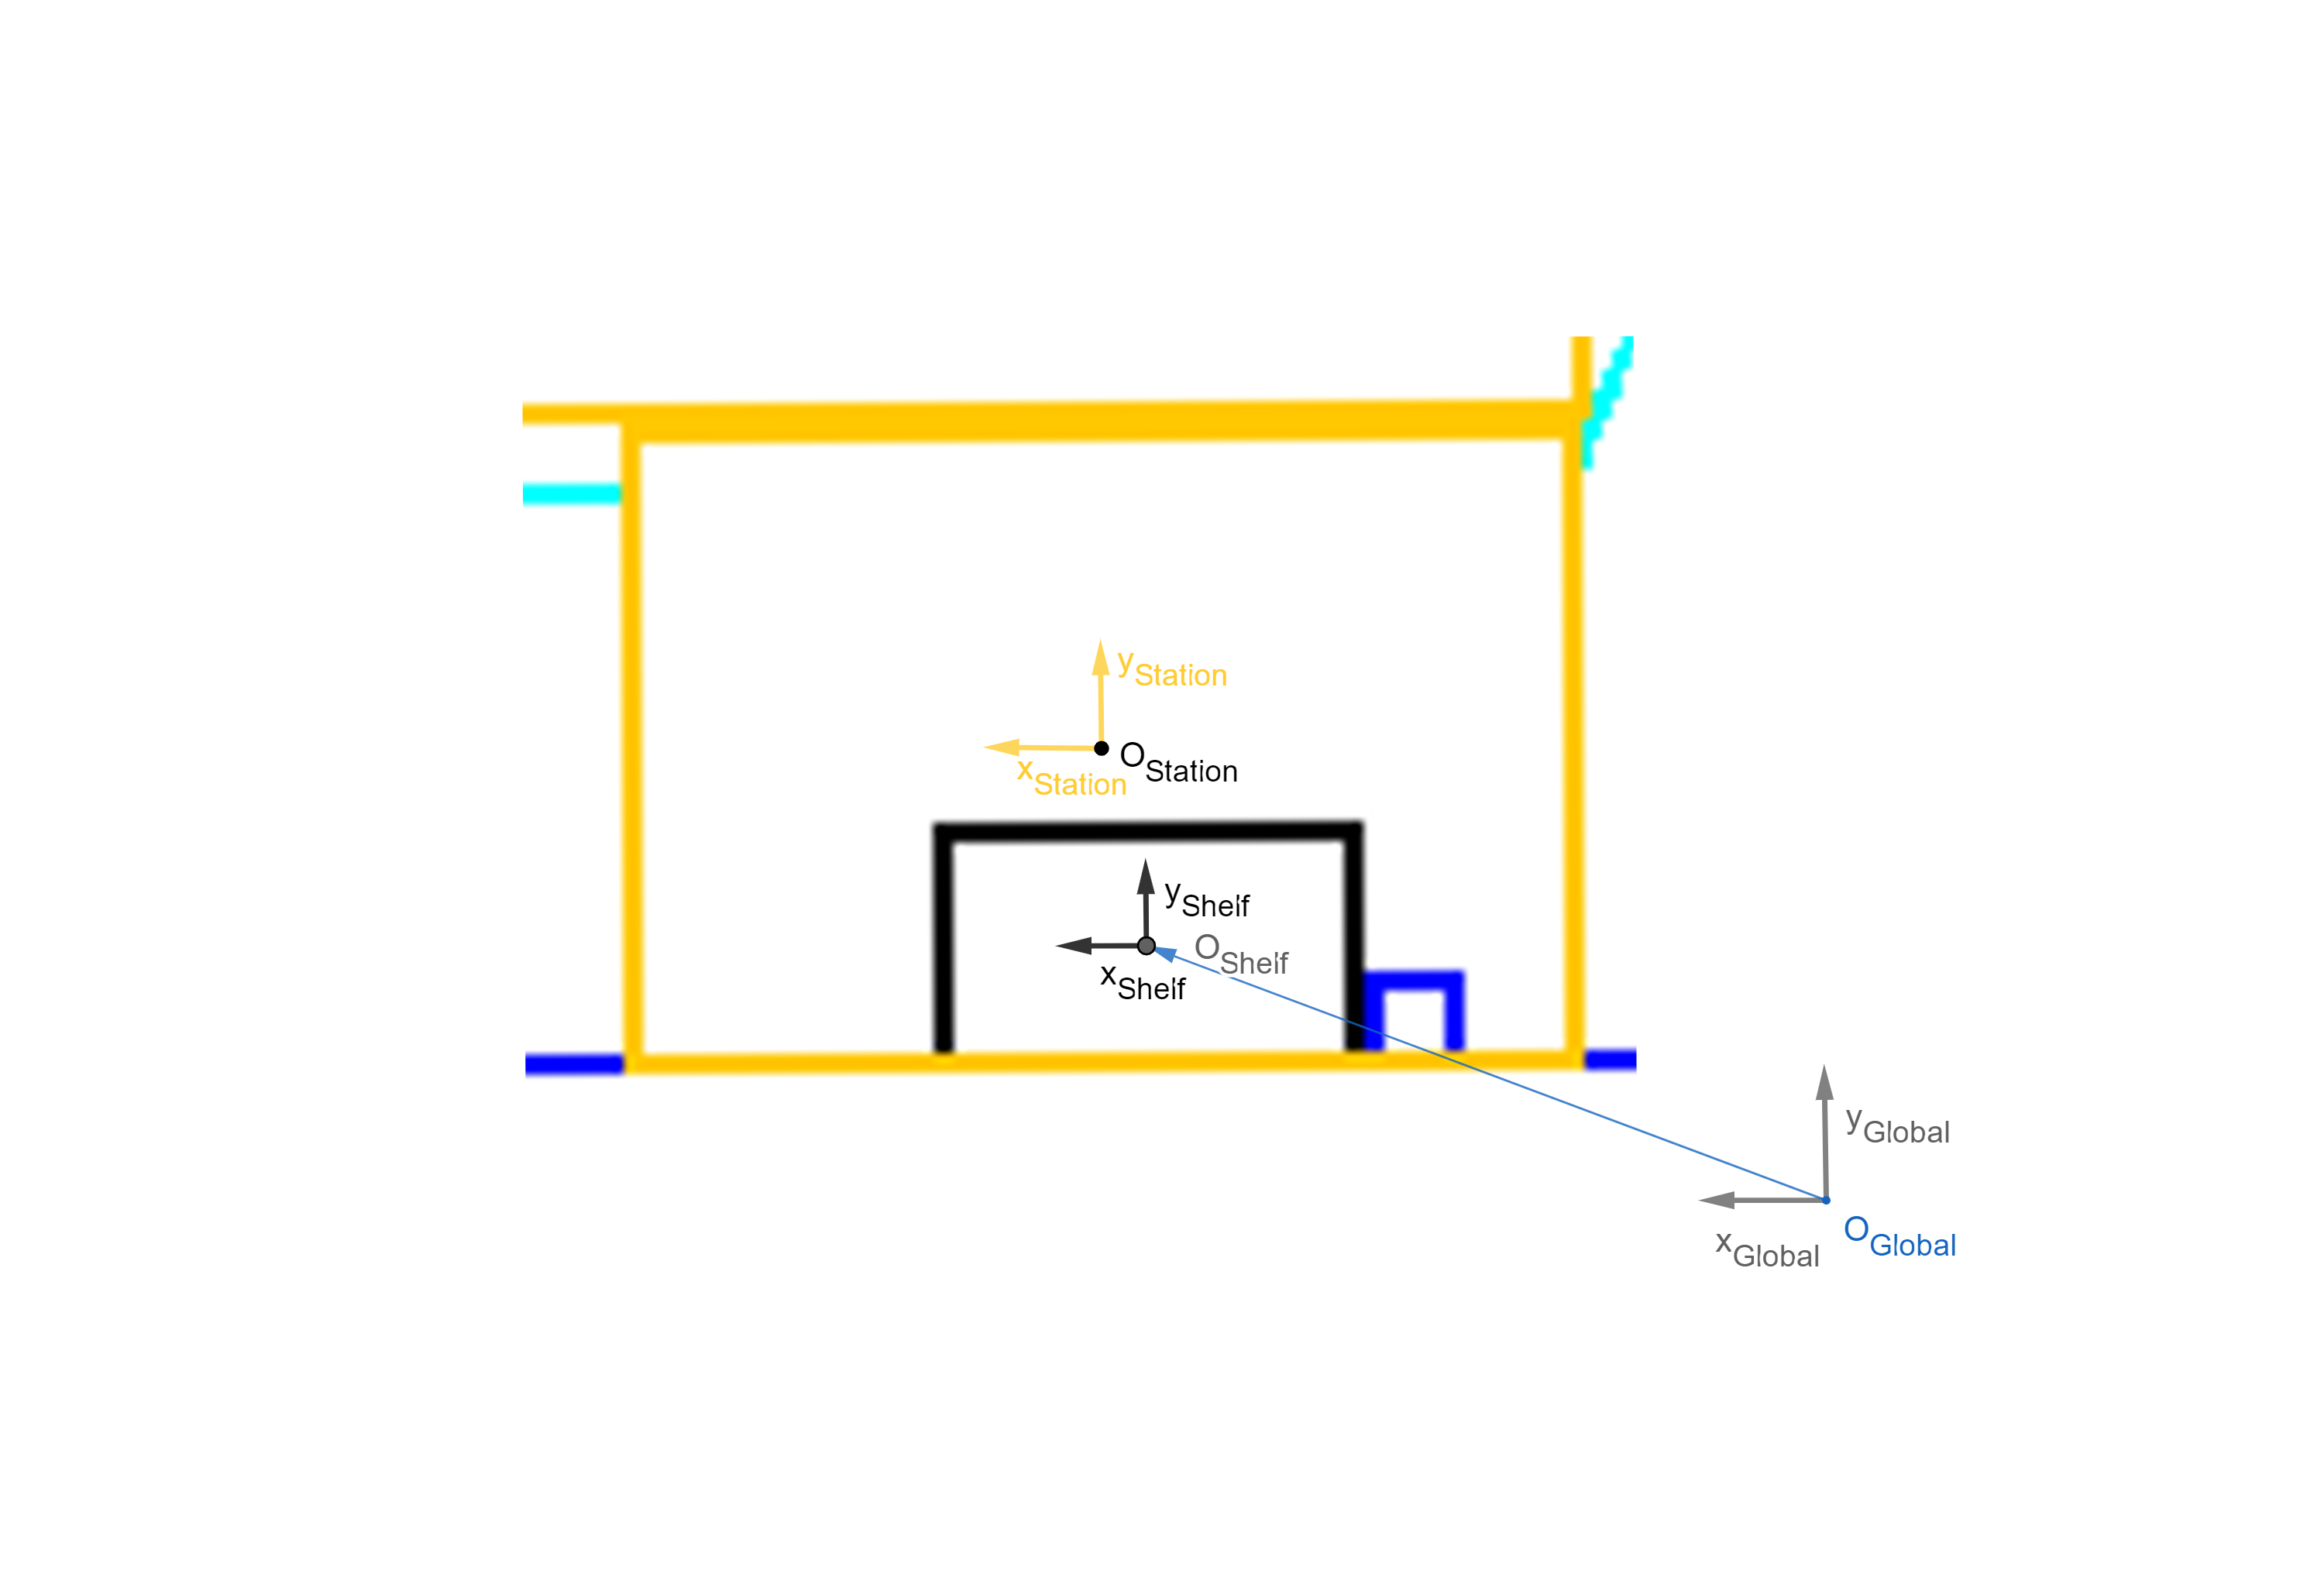
\includegraphics[width=5in]{images/Chap2/Fixed_frames.png}\\
        \caption{Station Simulation with added Station, Shelf, and Global (World) frames}
        \label{Station}
        \end{center}    
\end{figure}

It is measured as follows:
\begin{equation}
    T_{Shelf}^{Global} = 
    \begin{pmatrix}
    \cos(\theta) & -\sin(\theta) & t_x \\
    \sin(\theta) & \cos(\theta) & t_y \\
    0 & 0 & 1
    \label{shToGlob}
    \end{pmatrix}
    \end{equation}
    
    \noindent Where:
    
    \noindent $\theta$ is the rotation angle between the shelf and global frames. \\

    \noindent $t_x$ and $t_y$ are the translation components along the x and y axes, respectively.
    
    \vspace{1em} 
Now, the inverse transformation that will be used to change the coordinates from 
the global frame to the shelf frame is:
    
    \begin{equation}
    T_{Global}^{Shelf} = \left( T_{Shelf}^{Global} \right)^{-1}
    \end{equation}

The algorithm then iteratively transforms the station and shelf corners from global coordinates to shelf coordinates, 
storing the transformed corners in dedicated lists. 
The mathematical equation behind this transformation can be expressed as:

\begin{equation}
\begin{pmatrix}
x_{shelf} \\
y_{shelf} \\
1
\end{pmatrix}
=
T_{Global}^{Shelf}
\begin{pmatrix}
x_{global} \\
y_{global} \\
1
\end{pmatrix}
\end{equation}

Where:

\begin{equation}
\begin{pmatrix}
x_{shelf} \\
y_{shelf} \\
1
\end{pmatrix}
\end{equation}
is the transformed point in the shelf frame 

\begin{equation}
\begin{pmatrix}
x_{global} \\
y_{global} \\
1
\end{pmatrix}
\end{equation}
is the original point in the Global (World) frame

After the transformation, two subpolygons are created: one 
representing the Negative Y Subpolygon (Negative Y of the robot-related frame) ,(NegYsub\_polygon) and the other representing the 
Positive Y Subpolygon (Positive Y of the robot-related frame)
(PosYsub\_polygon). 
The subpolygons are data structures recognized by their global position and dimensions.
\newline \textbf{Definitions:}

\begin{itemize}
    \item \texttt{max\_st\_x}: Maximum x-coordinate of the station corners in the station frame.
    \item \texttt{min\_sh\_y}: Minimum y-coordinate of the shelf corners in the shelf frame.
    \item \texttt{SubPolygon\_Width}: Width of the subpolygon (previously measured)
    \item \texttt{SubPolygon\_Height}: Height of the subpolygon (previously measured)
\end{itemize}

The position of the sub-polygon is thus measured:
\begin{equation}
\text{SubPolygon.x} = \text{max\_sh\_x} + \frac{\text{SubPolygon\_Width}}{2}
\end{equation}
\begin{equation}
\text{SubPolygon.y} = \text{min\_sh\_y} + \frac{\text{SubPolygon\_Height}}{2}
\end{equation}

Then the subpolygon is transformed back to the global frame using the Transformation 
Matrix \Ref{shToGlob}:
\begin{equation}
\begin{pmatrix}
\text{GlobalSubPolygon.x} \\
\text{GlobalSubPolygon.y} \\
1
\end{pmatrix}
=
T_{shelf}^{Global}
\begin{pmatrix}
\text{SubPolygon.x} \\
\text{SubPolygon.y} \\
1
\end{pmatrix}
\end{equation}

For special cases like station3, where one of the subpolygons can be very narrow (lower than a 
certain threshhold), the algorithm omits it and generates only one subpolygon. 
The algorithm concludes by returning the created subpolygon(s), effectively segmenting the 
input areas into distinct, usable geometric entities.
The Pseudocode of the General Algorithm is given in Algorithm \Ref{alg:createSubpolygons}


\begin{figure}[H]
    \begin{center}
        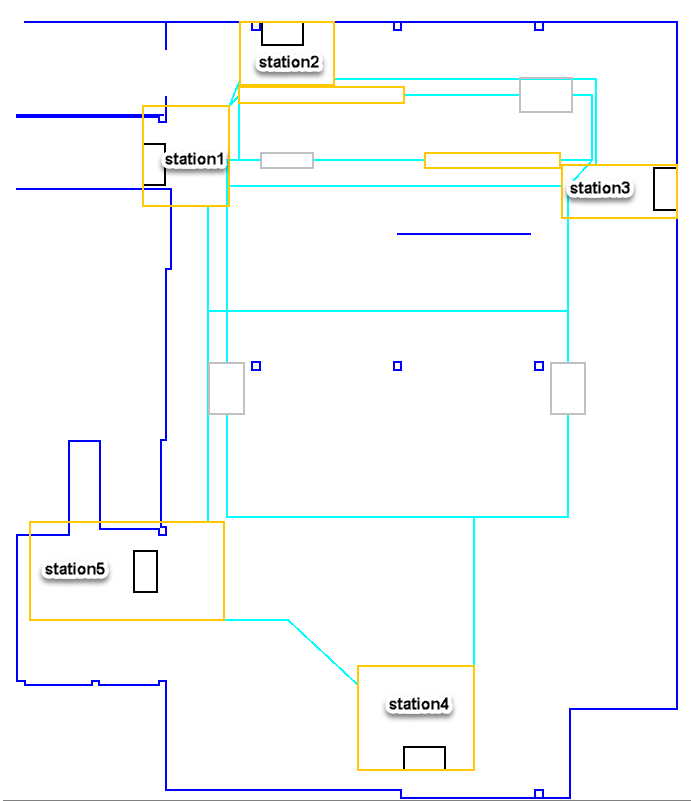
\includegraphics[width=4in]{images/Chap2/warehouse.png}\\
        \caption{Simulation of the stations in a warehouse}
        \label{warehouse}
        \end{center}    
\end{figure}

The colored elements in this figure are explained here:
\begin{itemize}
    \item Dark Blue outline: walls of the warehouse
    \item Yellow Rectancles marked as stations: Warehouse stations: Actions like picking up or 
    dropping are performed in specific locations inside the warehouse called 
    stations, examples of which are named \(station1\), \(station2\), and \(station3\) on the figure \Ref{move}.
    Each station is designed to support specific warehouse functions and their general mission
    is to facilitate and organize material handling operations. 
    Each station contains a \textbf{shelf} that contains the pallets to be picked or dropped. 
    \item Black rectangles: storage shelves (also called racks), where the  pallets and material are 
    stored. 
    \item Turquoise blue lines: Global paths that connect the stations.
    The truck takes these routes when navigating from a station to the other while avoiding 
    obstacles online if they occur.
    \item Gray rectangles are starting position of the truck around the warehouse. For instance,
    the truck can be placed at these positions before starting its autonomous navigation and 
    task fulfillment.

\end{itemize}



\noindent

\begin{algorithm}[H]
\caption{Creation of Subpolygons}\label{alg:createSubpolygons}
\KwData{station\_area, shelf\_area}
\KwResult{created two subpolygons}
\BlankLine
\textbf{Initialization}; \\
station\_corners, shelf\_corners $\gets$ GetCorners(station\_area, shelf\_area)\;
tm\_station\_corners, tm\_shelf\_corners $\gets$ empty lists\;
tm\_shelf2global $\gets$ GetTransMatrix(shelf\_area)\;
tm\_global2shelf $\gets$ InvertMatrix(tm\_shelf2global)\;
\ForEach{corner $\in$ station\_corners}{
    corner\_shelf $\gets$ TransformCorner(tm\_global2shelf, corner)\;
    tm\_station\_corners.append(corner\_shelf)\;
}
station\_corners\_shelf.append(tm\_station\_corners[0])\;
\ForEach{corner $\in$ shelf\_corners}{
    corner\_shelf $\gets$ TransformCorner(tm\_global2shelf, corner)\;
    tm\_shelf\_corners.append(corner\_shelf)\;
}
NegYsub\_subpolygon $\gets$ CreateNegYsubpolygon(tm\_station\_corners, tm\_shelf\_corners, tm\_shelf2global)\;
PosYsub\_subpolygon $\gets$ CreatePosYsubpolygon(tm\_station\_corners, tm\_shelf\_corners, tm\_shelf2global)\;
\Return{created two subpolygons}\;
\end{algorithm}
\noindent



\subsubsection{Results of the Station Partitioning}

In figure \ref{Station polygon} stands the simulated result processed using real station data: In purple and orange are 
the polygons, and in green the outer polygon represenst the station.
The station used is the Station \(Empty Pallets\) of the warehouse.
%TODO: write here 

\begin{figure}[H]
    \begin{center}
        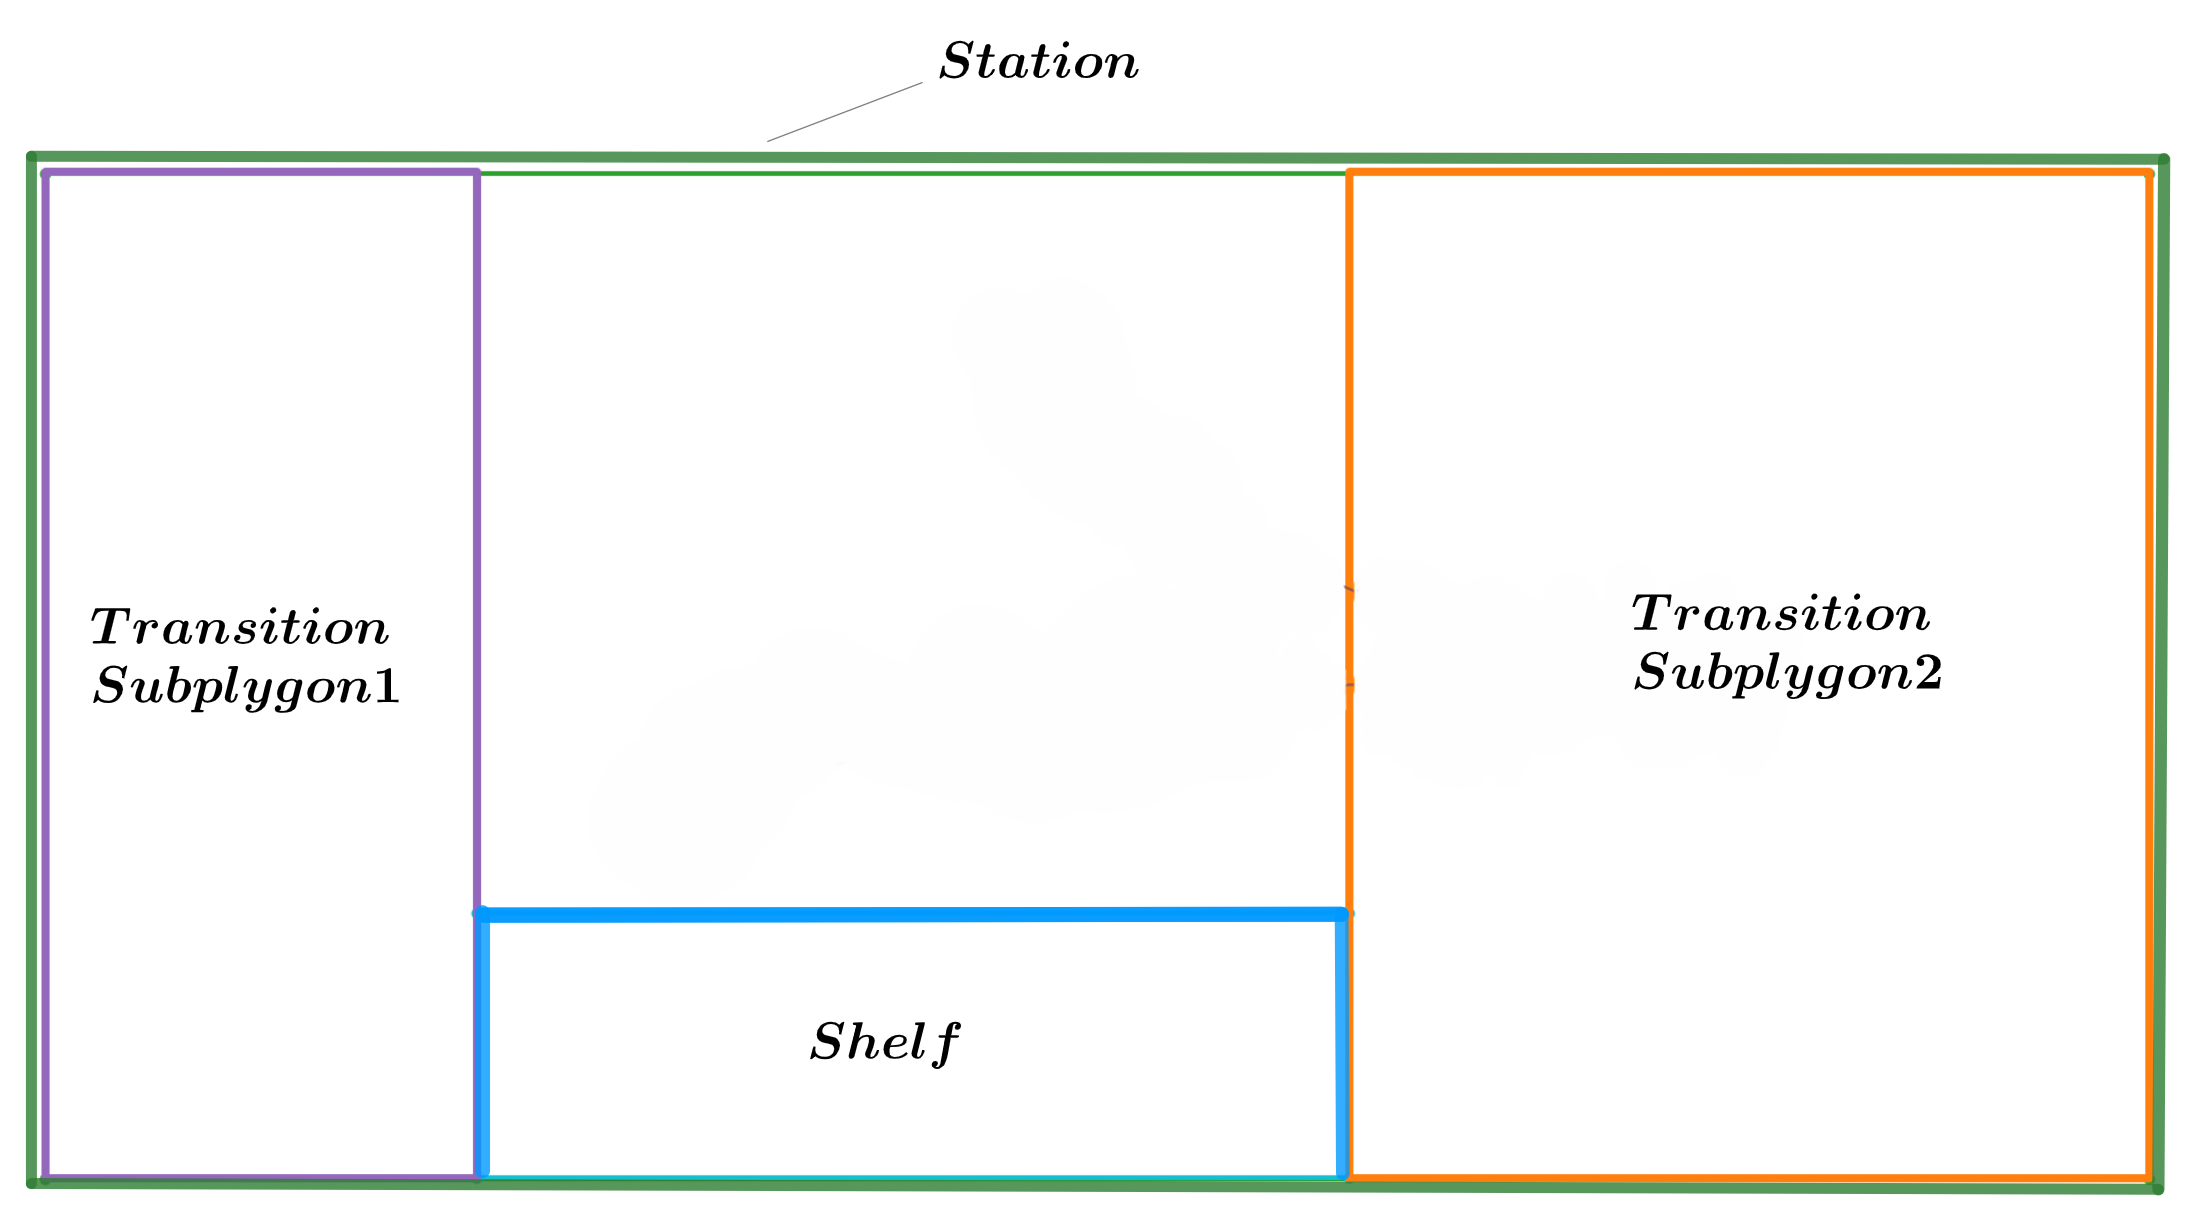
\includegraphics[width=4in]{images/Chap2/subpolygons.png}\\
        \caption{Partitioning: Station divided into subpolygons}
        \label{Station polygon}
        \end{center}    
\end{figure}


\subsection{Path creation}
This section details the methodology for path creation. \textbf{The input of this section are the polygons besides
the robot's position and the destination. The output is a spline-based path linking the robot to the destination with a 
driving direction change}.

\subsubsection{Choice of Path Creation Methodology}
The pattern path links the AMR at the start position to the transition position on the subpolygon then to the 
destination point as illustrated in figure \Ref{pattern}. 
The waypoints depicted on the simulation figure \ref{Orientation} 
are created relating to the 
Robot, the destination and the transition positions. In a simple scenario where no obstacles are present, orientation points 
are strategically added in front of the three key positions of the robot. These orientation points serve as reference markers 
that guide the robot's movement, particularly during the initial phase of acceleration or deceleration. When the robot starts 
to move, it follows a precise trajectory, either in a straightforward or straight-backward direction, depending on the 
intended driving direction. This straight-line motion ensures that the robot maintains stability and accuracy as it 
transitions from a stationary position to motion or vice versa, minimizing any unnecessary deviations or turns that could 
disrupt its path. The alignment with the orientation points helps the robot to consistently maintain a straight trajectory, 
which is crucial for precise navigation and control.
%TODO: remove white space from the next figures
\begin{figure}[H]
    \begin{center}
        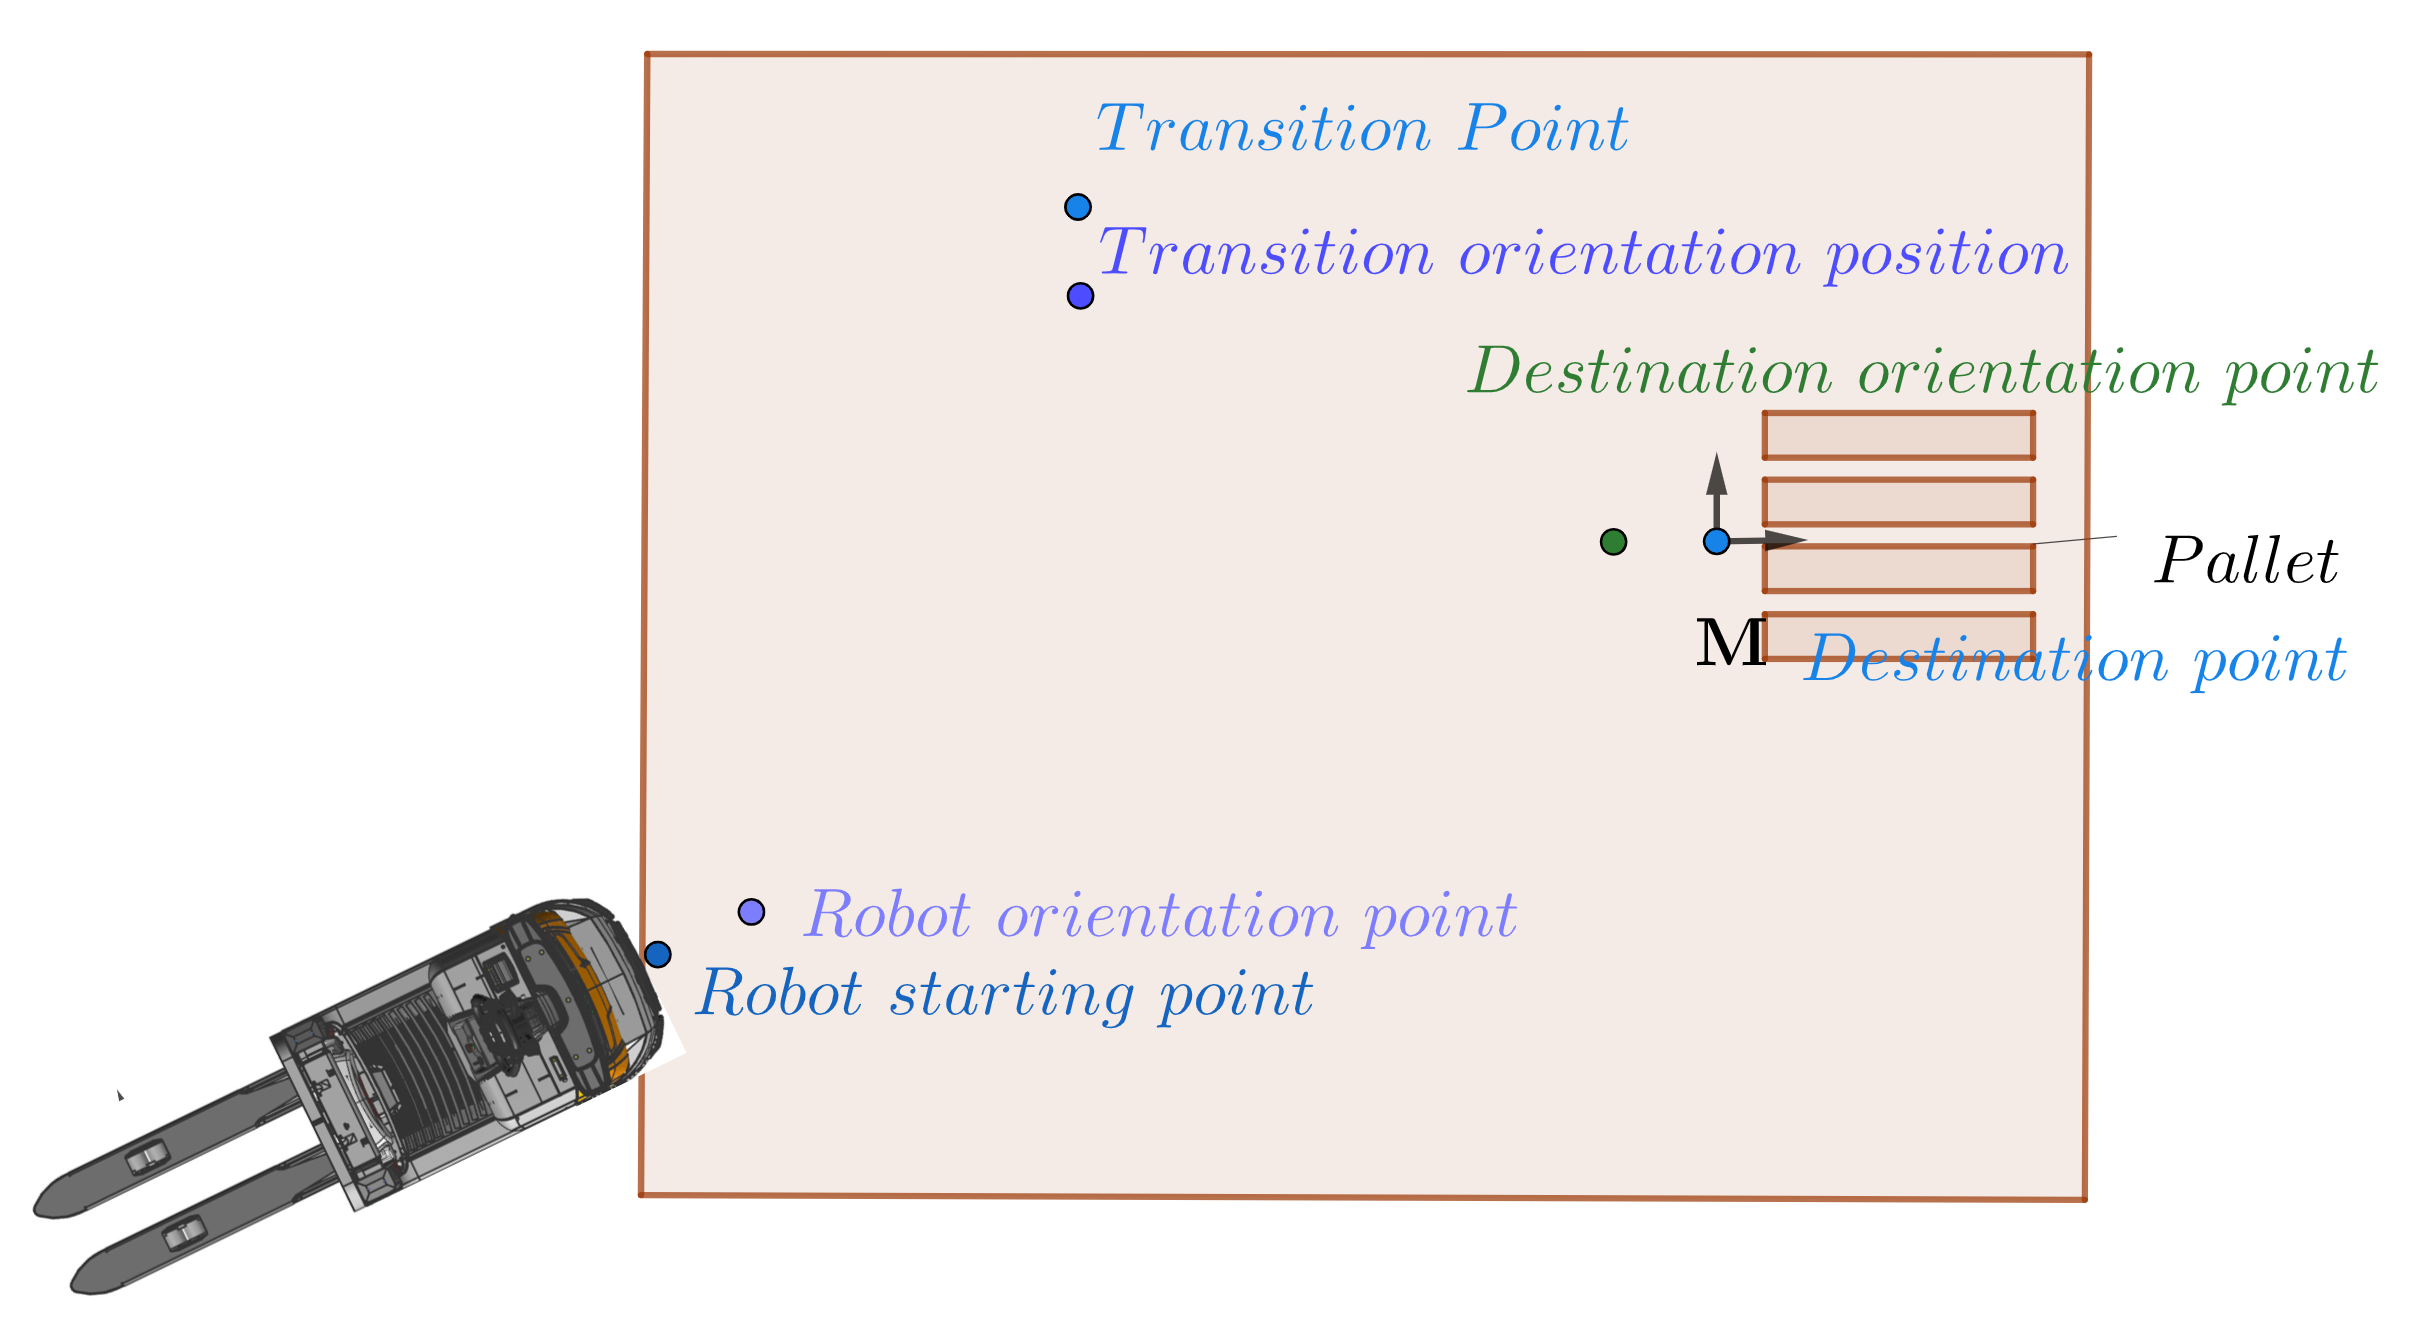
\includegraphics[width=5in]{images/Chap2/Orientation_points.png}\\
        \caption{Step2: Orientation Points creation using the 3 origin path points}
        \label{Orientation}
        \end{center}    
\end{figure}

The waypoints are then connected to form the path.
However, to obtain smooth paths there should be curved paths that connect waypoints seamlessly instead 
of simple vertices connection. 

Spline-based paths provide several key benefits for robotic navigation. They ensure smooth and continuous movement by 
creating curved paths that connect waypoints seamlessly. Unlike abrupt turns and sharply angled paths, this smoothness 
reduces wear on the robot and makes its movements more energy-efficient. Additionally, spline-based paths make it 
easier to control the robot in real-time, allowing for quick adjustments if the environment changes and preventing 
oscillations as a response to control corrections. Using mathematical 
equations to define these paths also makes it simple to calculate important 
properties like path length and curvature, helping the robot navigate efficiently and safely. 

\subsubsection{Spline Based Paths}
\subsubsubsection{Splines Applications in Robotics}
%How splines facilitate smooth and continuous trajectory planning.
Robots like AMRs in the intralogistics sector usually have mission to carry heavy loads. 
This property makes it risky to operate abrupt motion changes like stopping or turning.
These vehicles' motion planning requires precise control and detailed alignment to the 
kinematic constraints that they present \cite{R30}.
Given the mathematical nature of Splines, namely B-splines they ensure continuity of 
the first and second derivatives.
This continuity translates to smooth transitions of the resulting velocities and accelerations of the path
that the robot will follow. By having continuous velocity and acceleration, we make sure that the robot
achieves smooth transitions and speed changes. Furthermore, tracking, precise following and correct control
interventions are guaranteed allowing for precise navigation \cite{R30}. 

 
Although simple,
the connected waypoints approach comes with drawbacks like sub-optimal travel time, unoptimized long paths, 
and mechanical wear because of abrupt direction changes unlike curved paths \cite{R30}. The morphological 
difference in both paths is distinguished in figure \Ref{paths}. 
On the reader's left is a path of consequent vertices. This path has corner shaped turns which are rough to 
navigate for AMRs. The vehicle has to stop at the corner before taking the next vertice 
as the change in direction happens suddenly and not gradually.
On the right, the path is a curve controlled by the positions of the waypoints. 
The change in direction happens gradually and the navigation on this route is smoother than the previous.

\begin{figure}[H]
    \begin{center}
        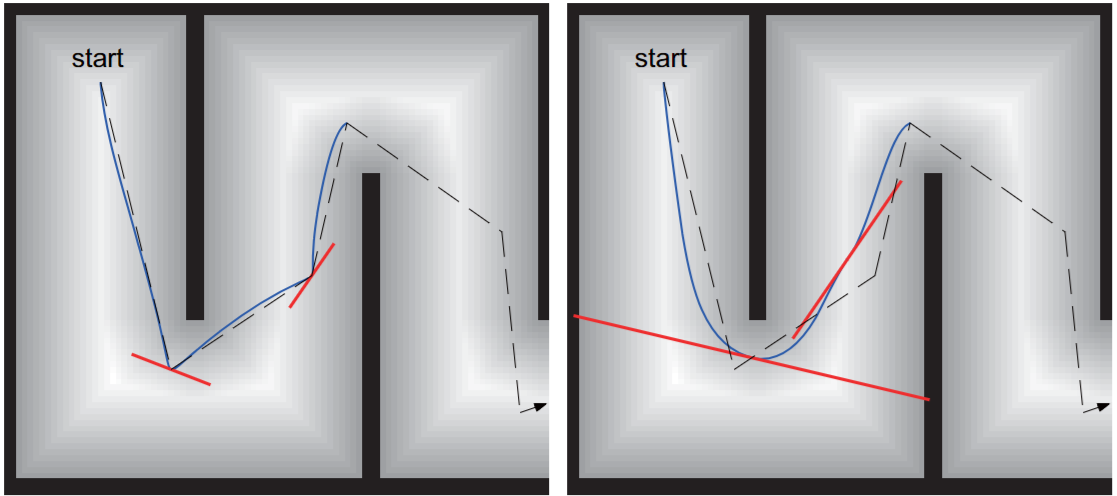
\includegraphics[width=4in]{images/Chap2/sharp-vs-curved-path.png}\\
        \caption{Morphological difference between a path connecting waypoints (left) and a curved path 
        (right) \cite{R30}}
        \label{paths}
    \end{center}
\end{figure}

Multiple approaches have been developed to introduce smooth transitions and turns into robot trajectories. 
One such method involves using Clothoid curves, which connect straight path segments with circular arcs 
to avoid abrupt changes in direction \cite{R31}. Originally introduced for designing highways and roads to 
ensure safe and comfortable driving for humans, Clothoids offer a gradual change in curvature.

However, when applied to robotics, Clothoid curves present certain drawbacks. These include the potential 
for discontinuities in curvature at the transitions, which can lead to jerky motions in robotic paths. 
Additionally, Clothoid-based paths can result in sub-optimal path lengths, as they may not be the shortest 
possible routes. Moreover, while circular arcs with constant radii are used in this approach, long
arcs lead to large curvatures, and can lead to loss of control and instability of the AMR , which can 
be impractical for mobile robots that require tighter turns 
and more precise control \cite{R31}.

%Techniques for smoothing rough paths generated by planners.
Migrating from a path with sharp angles to one with smooth curves can be effectively accomplished by 
using splines. The interpolation of the control points of the original path 
creates a smooth, continuous curve. By incorporating a convex hull around these control points, we 
ensure that the path does not deviate excessively from the desired points, thus avoiding potential 
collisions with obstacles \cite{R33}. The convex hull acts as a boundary that keeps the spline inside the limits of 
the control points that prametrize it (see figure \Ref{convex-hull}) and keeps the robot from straying 
too far, ensuring a safe and accurate trajectory \cite{R29}.

\begin{figure}[H]
    \begin{center}
        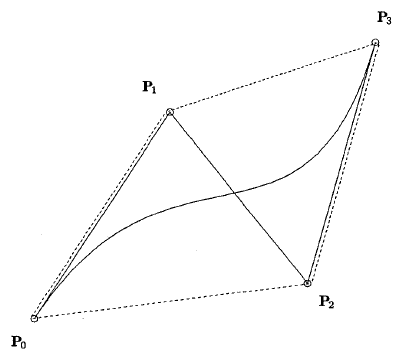
\includegraphics[width=3in]{images/Chap2/convex-hull.png}\\
        \caption{Convex hull contained Spline \cite{R29}}
        \label{convex-hull}
    \end{center}
\end{figure}

Splines are advantageous because they can accommodate various constraints such as curvature limits 
and minimum turning radii. These constraints are crucial in many applications, including robotics 
and vehicle navigation, where maintaining a smooth path is essential for stability and control. 
By adjusting the spline parameters, it is possible to design paths that meet specific requirements, 
ensuring that the resulting trajectory is not only smooth but also feasible given the physical and 
operational constraints \cite{R30}.

In scenarios involving obstacle avoidance, splines can be blended or connected to create a seamless 
path while circumventing obstacles. This blending technique allows for the integration of different 
spline segments into a continuous trajectory, ensuring that the path remains clear of obstacles. 
By carefully adjusting the blend points and ensuring smooth transitions between splines, it is 
possible to navigate complex environments safely and efficiently. This approach combines the 
advantages of smooth path planning with effective obstacle avoidance.

%Case studies of spline-based trajectory planning in autonomous vehicles.

A notable case study of splines integration in solving path planning problems, is a research conducted 
by B. Lau et al. \cite{R30} that aims to develop a time optimal solution while considering the kinodynamic 
properties of a mobile robot. They used a global planner to generate straight-line paths and minimize time 
of travel. Then, they  integrated splines to join the resulting path segments in a smooth and continuous 
way and replan in case of unprecedented collisions. The results show that our motion planning system works 
well in both real and simulated settings. It created smooth and accurate paths, with an average positional 
error of about 1 cm and a velocity error of less than 2 cm/s. The optimization process improved travel 
time by 31\% compared to initial paths. The system also handled dynamic environments, like crowded trade 
shows, and adjusted smoothly when localization errors occurred by updating the path as needed. Overall, 
it performed reliably, navigating precisely and adapting effectively to changes and errors.

In general, Splines are an effective tool that centralizes advantages related to path smoothness,
simplicity of constraining the path according to the kinodynamic properties and mechanical
limitations of the mobile robot like limiting the curvature, and allowing for safe and smooth
speed and direction changes. These properties accommodate simple manipulation of splines for
path planning and tracking of path properties. As an illustration, it is possible to measure the
spline’s features like curvature or approximate its length.

\subsubsubsection{Splines Mathematical concepts}

In mathematics and computer graphics, a \textbf{curve} is a continuous and smooth flowing line without 
sharp angles \Ref{R29}. 
It can be defined parametrically or implicitly and represents a path that can be traced by a moving point.
A curve can be defined using a parameter 
\(u\), where \(u\)varies over an interval, and the coordinates of the curve are given by functions of:
\begin{equation}
    C(u) = (x(u), y(u)) \quad \text{given} \quad a \leq u \leq b \label{eq:curve}
\end{equation}

The circle is an example of a curve where:

\hspace*{-1cm} % Adjust the value as needed
\begin{align}
    x(u) &= \cos(u) \\
    y(u) &= \sin(u) \quad \text{given} \quad 0 \leq u \leq \frac{\pi}{2}     \cite{R29}
\end{align}

whereas, the implicit form of the circle would be:
\begin{equation}
    (x - h)^2 + (y - k)^2 = r^2
\end{equation}

where \((h,k)\) is the center and \(r\) is the radius.


Parametric curves have a clear direction (from C(a) to C(b)), which implicit curves lack. This makes 
it simpler to create ordered sequences of points along a parametric curve. Additionally, the parametric 
form is more intuitive for designing and modeling shapes on a computer, as the coefficients in many 
parametric functions (such as Bezier and B-Splines) carry geometric significance. This results in 
user-friendly design techniques and algorithms that are numerically stable \cite{R28}. 
However, using one polynome-curves is inadequate as it is not possible to represent complex shapes, certain 
curve changes, and fitting the needed points. 
The solution is to use piecewise polynomial curves of degree \((n-1)\) for example if we need to integrate
\(n\) data points \cite{R29}.

Polynomials are a commonly used type of function in robotics because they can be easily differentiated 
and are less prone to numerical rounding errors (known as floating point errors). Although they cannot 
represent every geometric curve, polynomials can usually approximate them with sufficient accuracy. 

Using classical polynomial functions or their derivatives in Bézier form is mathematically equivalent. 
This means that any curve described using standard polynomials can be transformed into a Bézier curve, 
and vice versa. However, when it comes to geometric modeling—especially in applications like computer 
graphics or robotics—the Bézier form is often preferred. This preference is due to the fact that the 
coefficients in the standard polynomial form (also known as the power basis form) don't offer much 
information about the curve's actual shape, making it harder to intuitively control and adjust the 
curve. In contrast, the coefficients in the Bézier form -the control points- directly influence the 
shape of the curve, in a visually meaningful way, making it easier to understand and manipulate 
as shown in equation \Ref{Bezier curve} \cite{R28}. 

\begin{equation}
    C(u) = \sum_{i=0}^{n} B_{i,n}(u) \mathbf{P}_i \quad \text{with } 0 \leq u \leq 1 \label{Bezier curve}
\end{equation}

The basis function \( B_{i,n}(u) \) is called the Bernstein polynomial of degree \( n \) and follows the equation

\begin{equation}
    B_{i,n}(u) = \frac{n!}{i!(n - i)!} \cdot u^i \cdot (1 - u)^{n - i} \label{}
\end{equation}

In this context, the Bernstein polynomial is a fundamental component. 
The basis function \( B_{i,n}(u) \) is used to determine how much influence each control 
point \( \mathbf{P}_i \) has on the shape of the Bézier curve.

The geometric coefficients \( \mathbf{P}_i \) are known as control points, and they define 
the shape of the polynomial curve. In many applications, such as mapping trajectories, 
a large number of control points is needed \cite{R28}.
Furthermore, in the Bézier form, the continuity of the curve depends on the placement of 
control points. This means if you want to change the shape of part of the curve while keeping 
the rest smooth, you can't easily do so because changing one part affects the whole curve \cite{R29}.

Instead, a more effective curve representation can be expressed as:

\begin{equation}
    C(u) = \sum_{i=0}^{n} N_i(u) \mathbf{P}_i
\end{equation}

where:
\begin{itemize}
    \item \( \mathbf{P}_i \): the control points
    \item \( N_i(u) \): the piecewise polynomial functions
\end{itemize}
The continuity of the curve is determined by these basis functions, allowing for flexible modification of 
control points without affecting the curve's smoothness \cite{R29}.

The basis functions for B-splines are defined recursively. For a given degree \( p \) and a set of non-decreasing knot values 
\( \{ u_i \} \), the basis functions \( N_{i,p}(u) \) can be defined as:

\begin{equation}
    N_{i,0}(u) = 
\begin{cases} 
1 & \text{if } u_i \leq u < u_{i+1} \\
0 & \text{otherwise}
\end{cases}
\end{equation}

\begin{equation}
N_{i,p}(u) = \frac{u - u_i}{u_{i+p} - u_i} N_{i,p-1}(u) + \frac{u_{i+p+1} - u}{u_{i+p+1} - u_{i+1}} N_{i+1,p-1}(u)
\end{equation}


With:
\begin{itemize}
    \item \( u \) is the parameter along the curve.
    \item \( u_i \) are the knot values, which divide the parameter range into intervals.
    \item \( N_{i,p}(u) \) are the B-spline basis functions of degree \( p \).
\end{itemize}

In figure \Ref{NURBS} stands an example of a spline (Red Curve) generated through setting random 
control points (Green squares) using th NURBS generator \cite{R32}. 

\begin{figure}[H]
    \begin{center}
    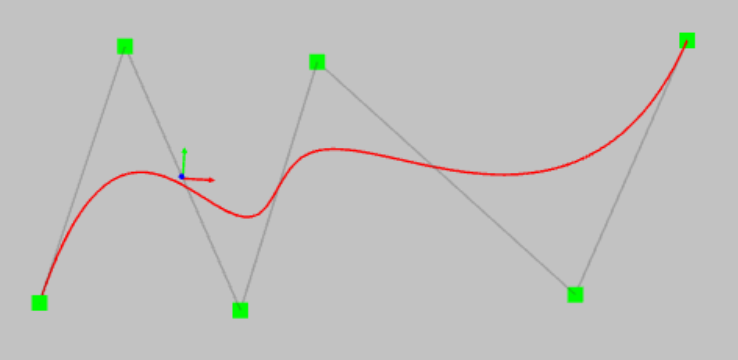
\includegraphics[width=4in]{images/Chap2/control-spline.png}\\
    \caption{NURBS spline example.\\
    \textbf{Green}: Control points\\
    \textbf{Red}: NURBS spline}
    \label{NURBS} 
    \end{center}
\end{figure}

Due to their local control and numerical stability, B-splines are preferred over other spline types. 
This means that modifying a single control point only affects a localized portion of the curve, making 
them easier to manipulate and less prone to numerical errors.
B-Splines will be used for the Creation of the paths for this work.

\subsubsection{Implementation of the Pattern Path Creation Approach}

Path creation comes after the creation of the subpolygons. After a transitioning point is chosen (see next section,
Path optimization), the waypoints are created. 

Then, the orientaion points are interpolated to create the spline-based path. Given the need to create the driving direction 
change as a straight section of the path, two different splines will be interpolated using 4 waypoints each:
\begin{itemize}
    \item The first spline interpolates the starting points then the transition points.
    \item The second spline interpolates the transition points then the destination points.
\end{itemize}

By doing so, two connected splines are obtained. Then they are merged together in the same path data structure to 
form one path. The first spline is driven in opposite direction driving, the second in main direction driving. 
The transition section at the polygon enables the robot to have an orientation that facilitates changing the driving direction
as given by figure \Ref{transition}.



\begin{figure}[H]
    \begin{center}
        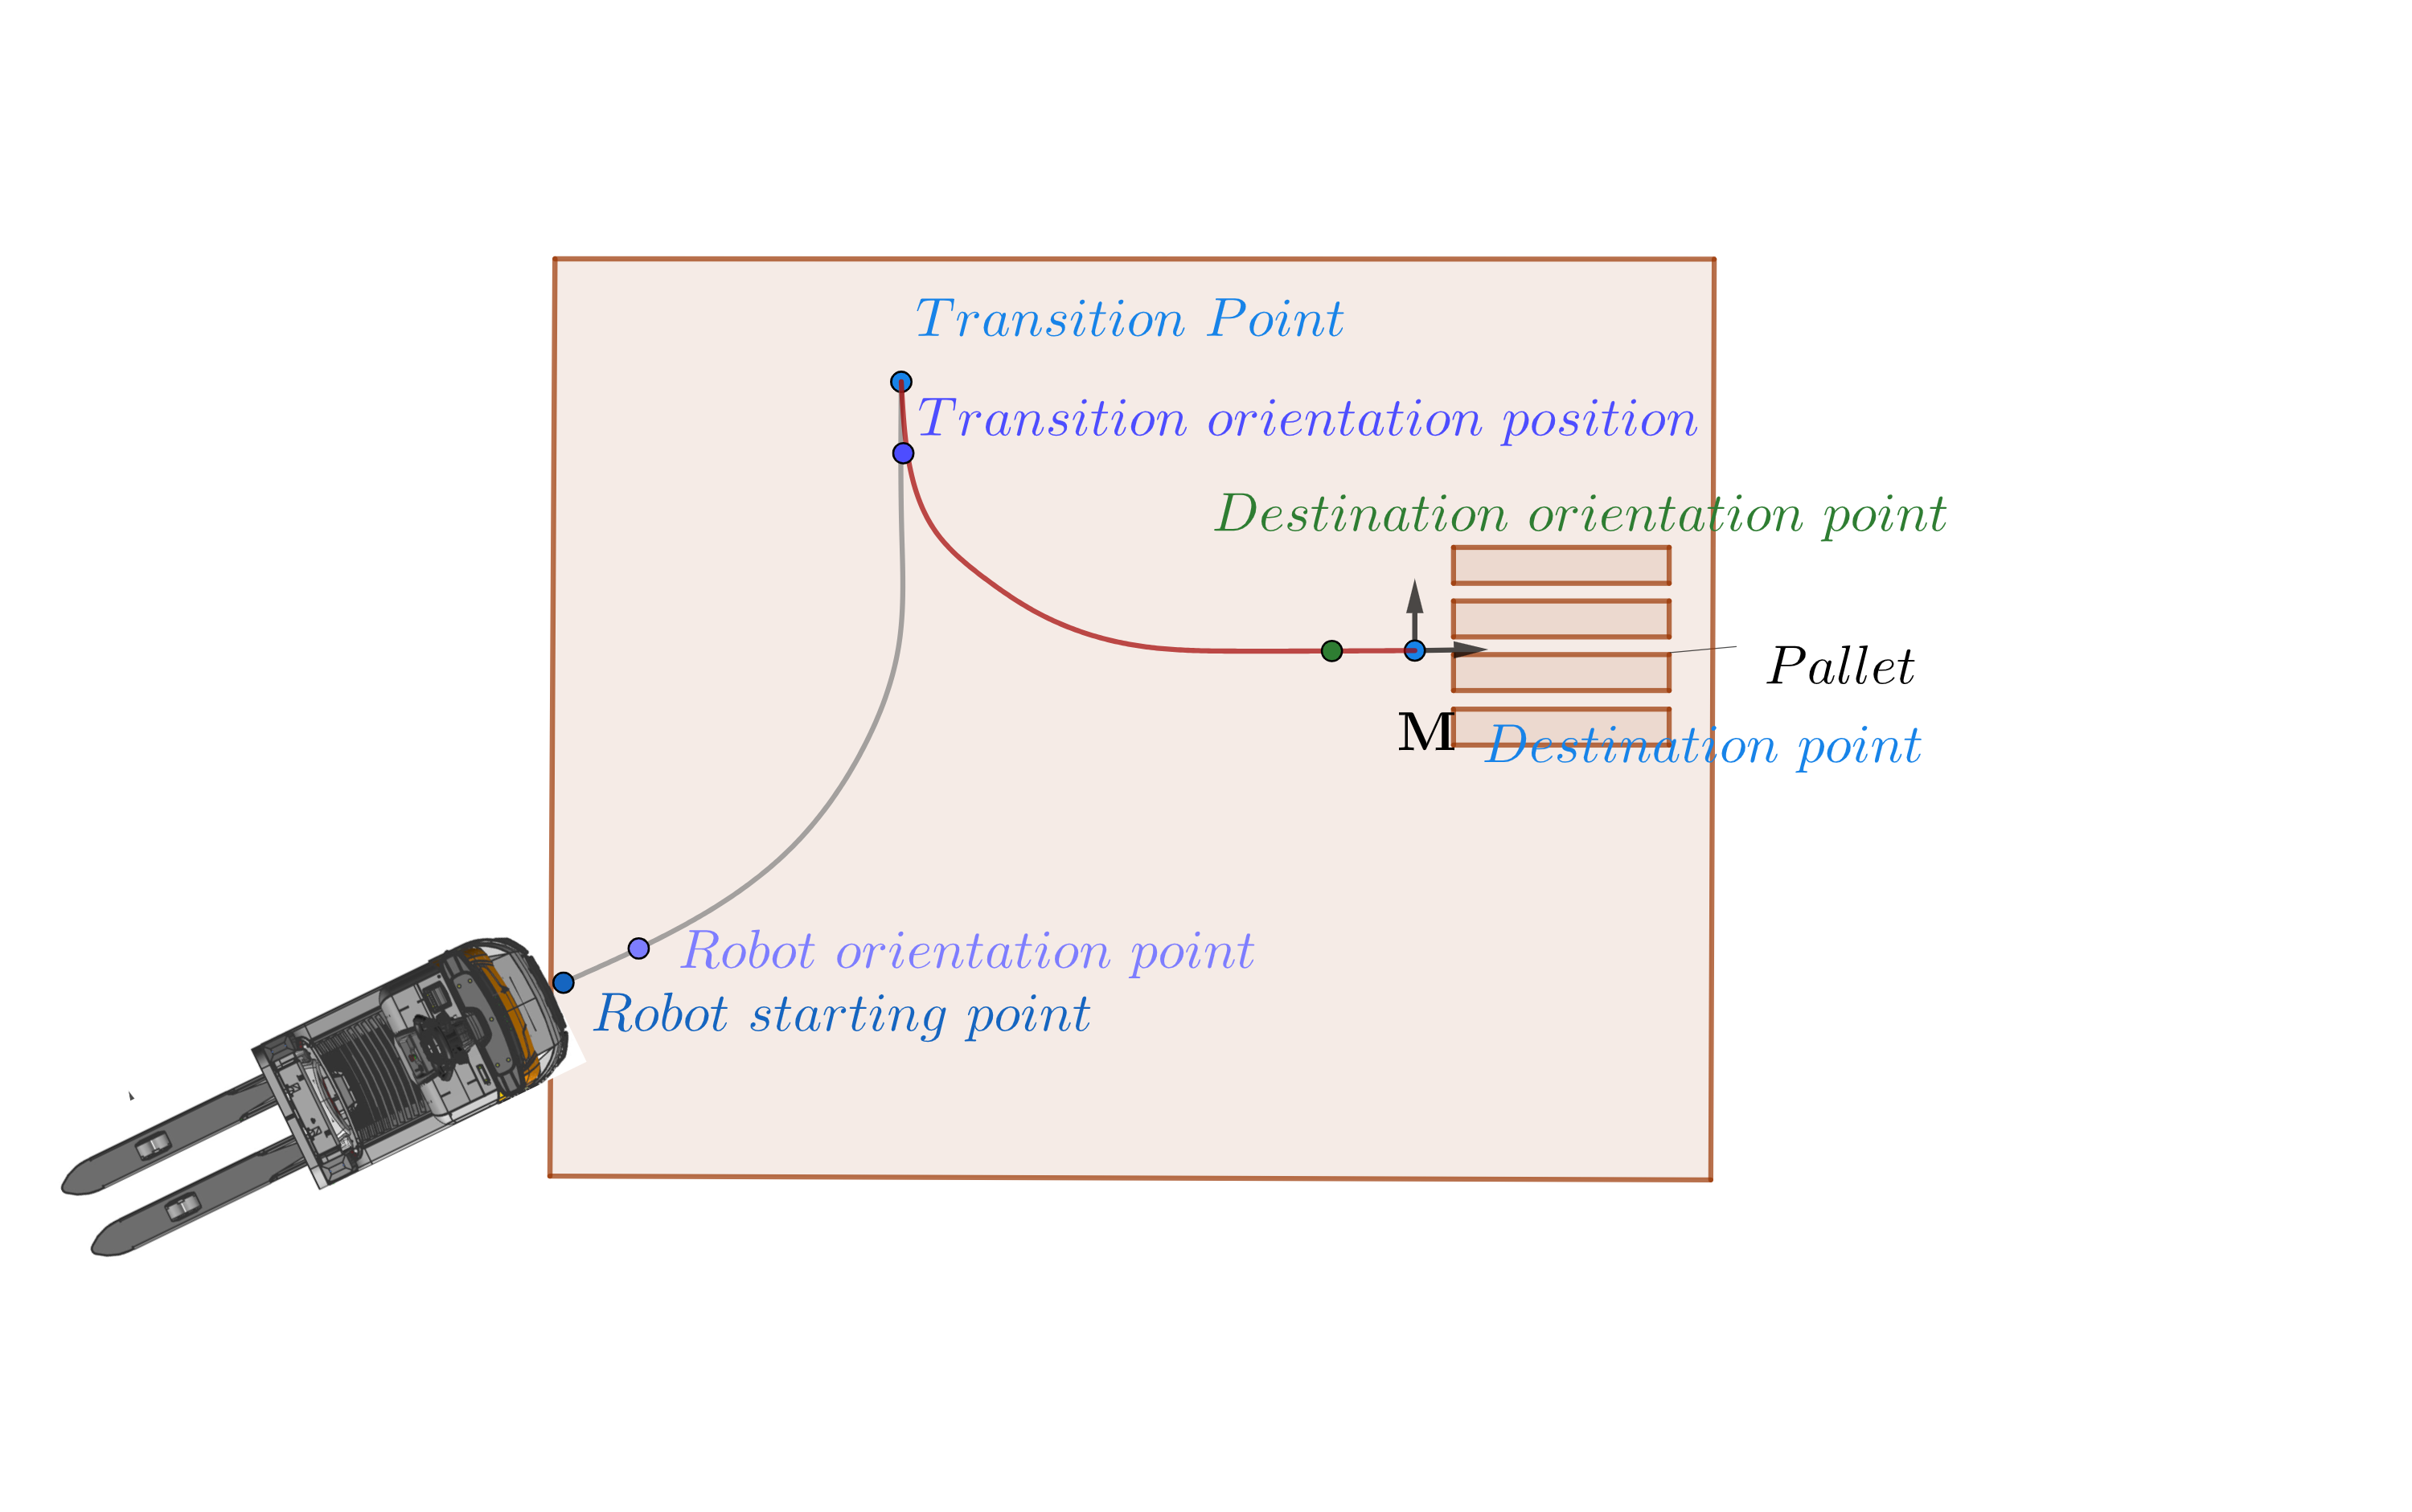
\includegraphics[width=5in]{images/Chap2/Orientation_points_with_spline.png}\\
        \caption{Step3: Interpolation of the waypoints and creation of the spline-based paths}
        \label{Spline ori}
        \end{center}    
\end{figure}

\begin{figure}[H]
    \begin{center}
        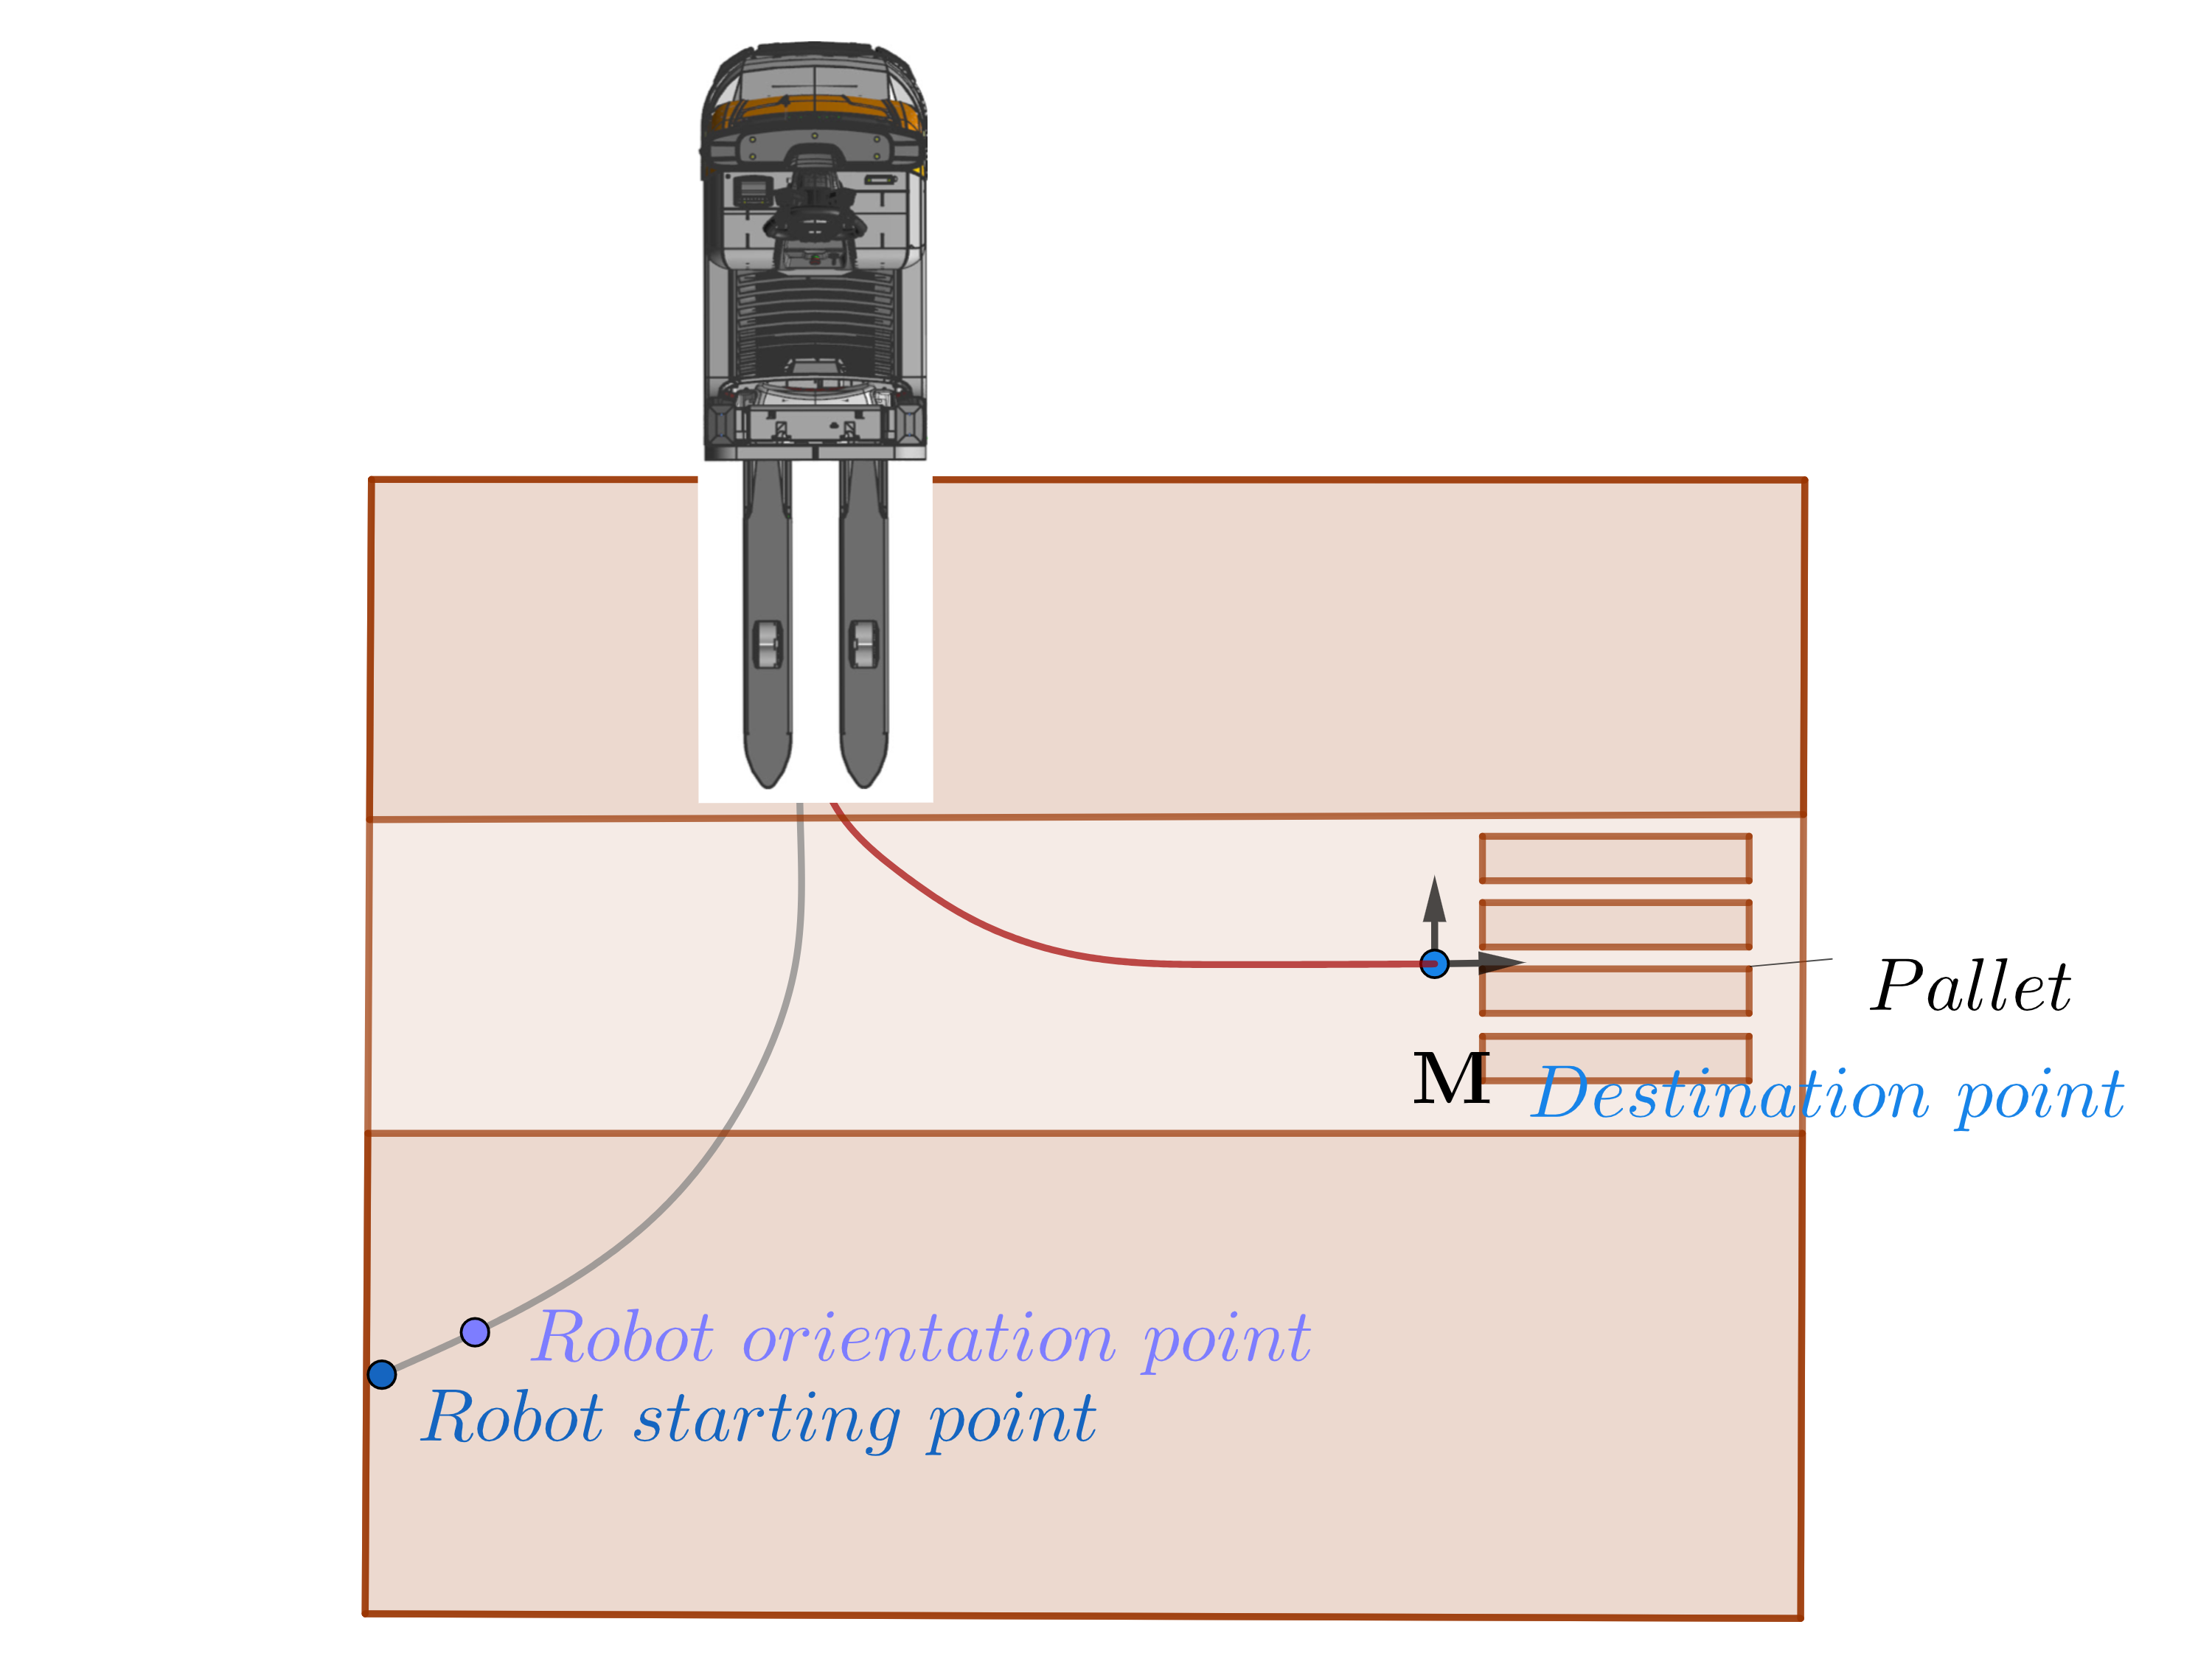
\includegraphics[width=5in]{images/Chap2/truck_transition.png}\\
        \caption{Robot at the transition position}
        \label{transition}
        \end{center}    
\end{figure}

The interpolation of the waypoints and the manipulation of splines is through The Spline Library integarted in 
the RACK framework (See RACK section%TODO add rack section
). The library provides tools to construct splines through several methods like interpolating points or blending two or more splines 
together and retrieve their features by segmeting the splines and calculating length and curvature for instance.
The result is a structure of coordinates through which passes the spline. 
The Algorithm of the approach to create a spline is explained in Pseudo code \Ref{alg:createSplines}.
The algorithm first acquires the waypoints to be interpolated. Then it creates the curve 
and measures the minimu and maximum parameter values from the knot vector which are used to evaluate 
the curve but also to retrieve relevant data about the splines like positions. It guides the exploration
of the spline. Besides, the spline length and cumulated curvature change are retrieved. 
The curvature change supervises the abrupt changes in curvature in segment curves of the whole spline.
Finally a number of positions belonging to the spline is retrieved and transfered to the path data structure,
this is where the resulting spline is transformed into a path that the robot can follow.

To fulfill the goal of path accuracy and precise docking of the target shelf or pallet, 
The path is create in the pallet frame. 
Once the AMR enters the station, it detects the shelf through the reflectors placed on 
the sides of the shelf marked in orange on figure \Ref{pattern}, which allows for 
real and accurate detection of the shelf. The pallet location is known through the shelf properties.
Then, transformation matrix are calculated using the reflectors positions in the robot 
$_{ }^{Robot}\text{ReflectorPos}$
and 
the pallet position in the Reflectors $_{ }^{Reflector}\text{PalletPos}$ to create the pattern path 
in the goal's frame:
The transformation matrix can be expressed as:

\begin{equation}
T_{Robot}^{Pallet} = T_{Reflector}^{Pallet} \cdot T_{Robot}^{Reflector}
\end{equation}

The transformation matrices and their inverses are represented as follows:

\begin{equation}
T_{Reflector}^{Pallet} = \left( T_{Pallet}^{Reflector} \right)^{-1}
\end{equation}

\begin{equation}
T_{Robot}^{Reflector} = \left( T_{Reflector}^{Robot} \right)^{-1}
\end{equation}

The transformation matrix from the pallet frame to the reflector frame is given by:

\begin{equation}
T_{Pallet}^{Reflector} = 
\begin{pmatrix}
\cos(\alpha) & -\sin(\alpha) & Pallet_{x}^{Reflector} \\
\sin(\alpha) & \cos(\alpha) & Pallet_{y}^{Reflector} \\
0 & 0 & 1
\end{pmatrix}
\end{equation}

Similarly, the transformation matrix from the reflector frame to the robot frame is:

\begin{equation}
T_{Reflector}^{Robot} = 
\begin{pmatrix}
\cos(\beta) & -\sin(\beta) & Reflector_{x}^{Robot} \\
\sin(\beta) & \cos(\beta) & Reflector_{y}^{Robot} \\
0 & 0 & 1
\end{pmatrix}
\end{equation}

Where:
\begin{itemize}
    \item \( \alpha \) is the orientation angle of $Pallet^{Reflector}$
    \item \( \beta \) is the orientation angle of $Reflector^{Robot}$
\end{itemize}



\begin{figure}[H]
    \begin{center}
        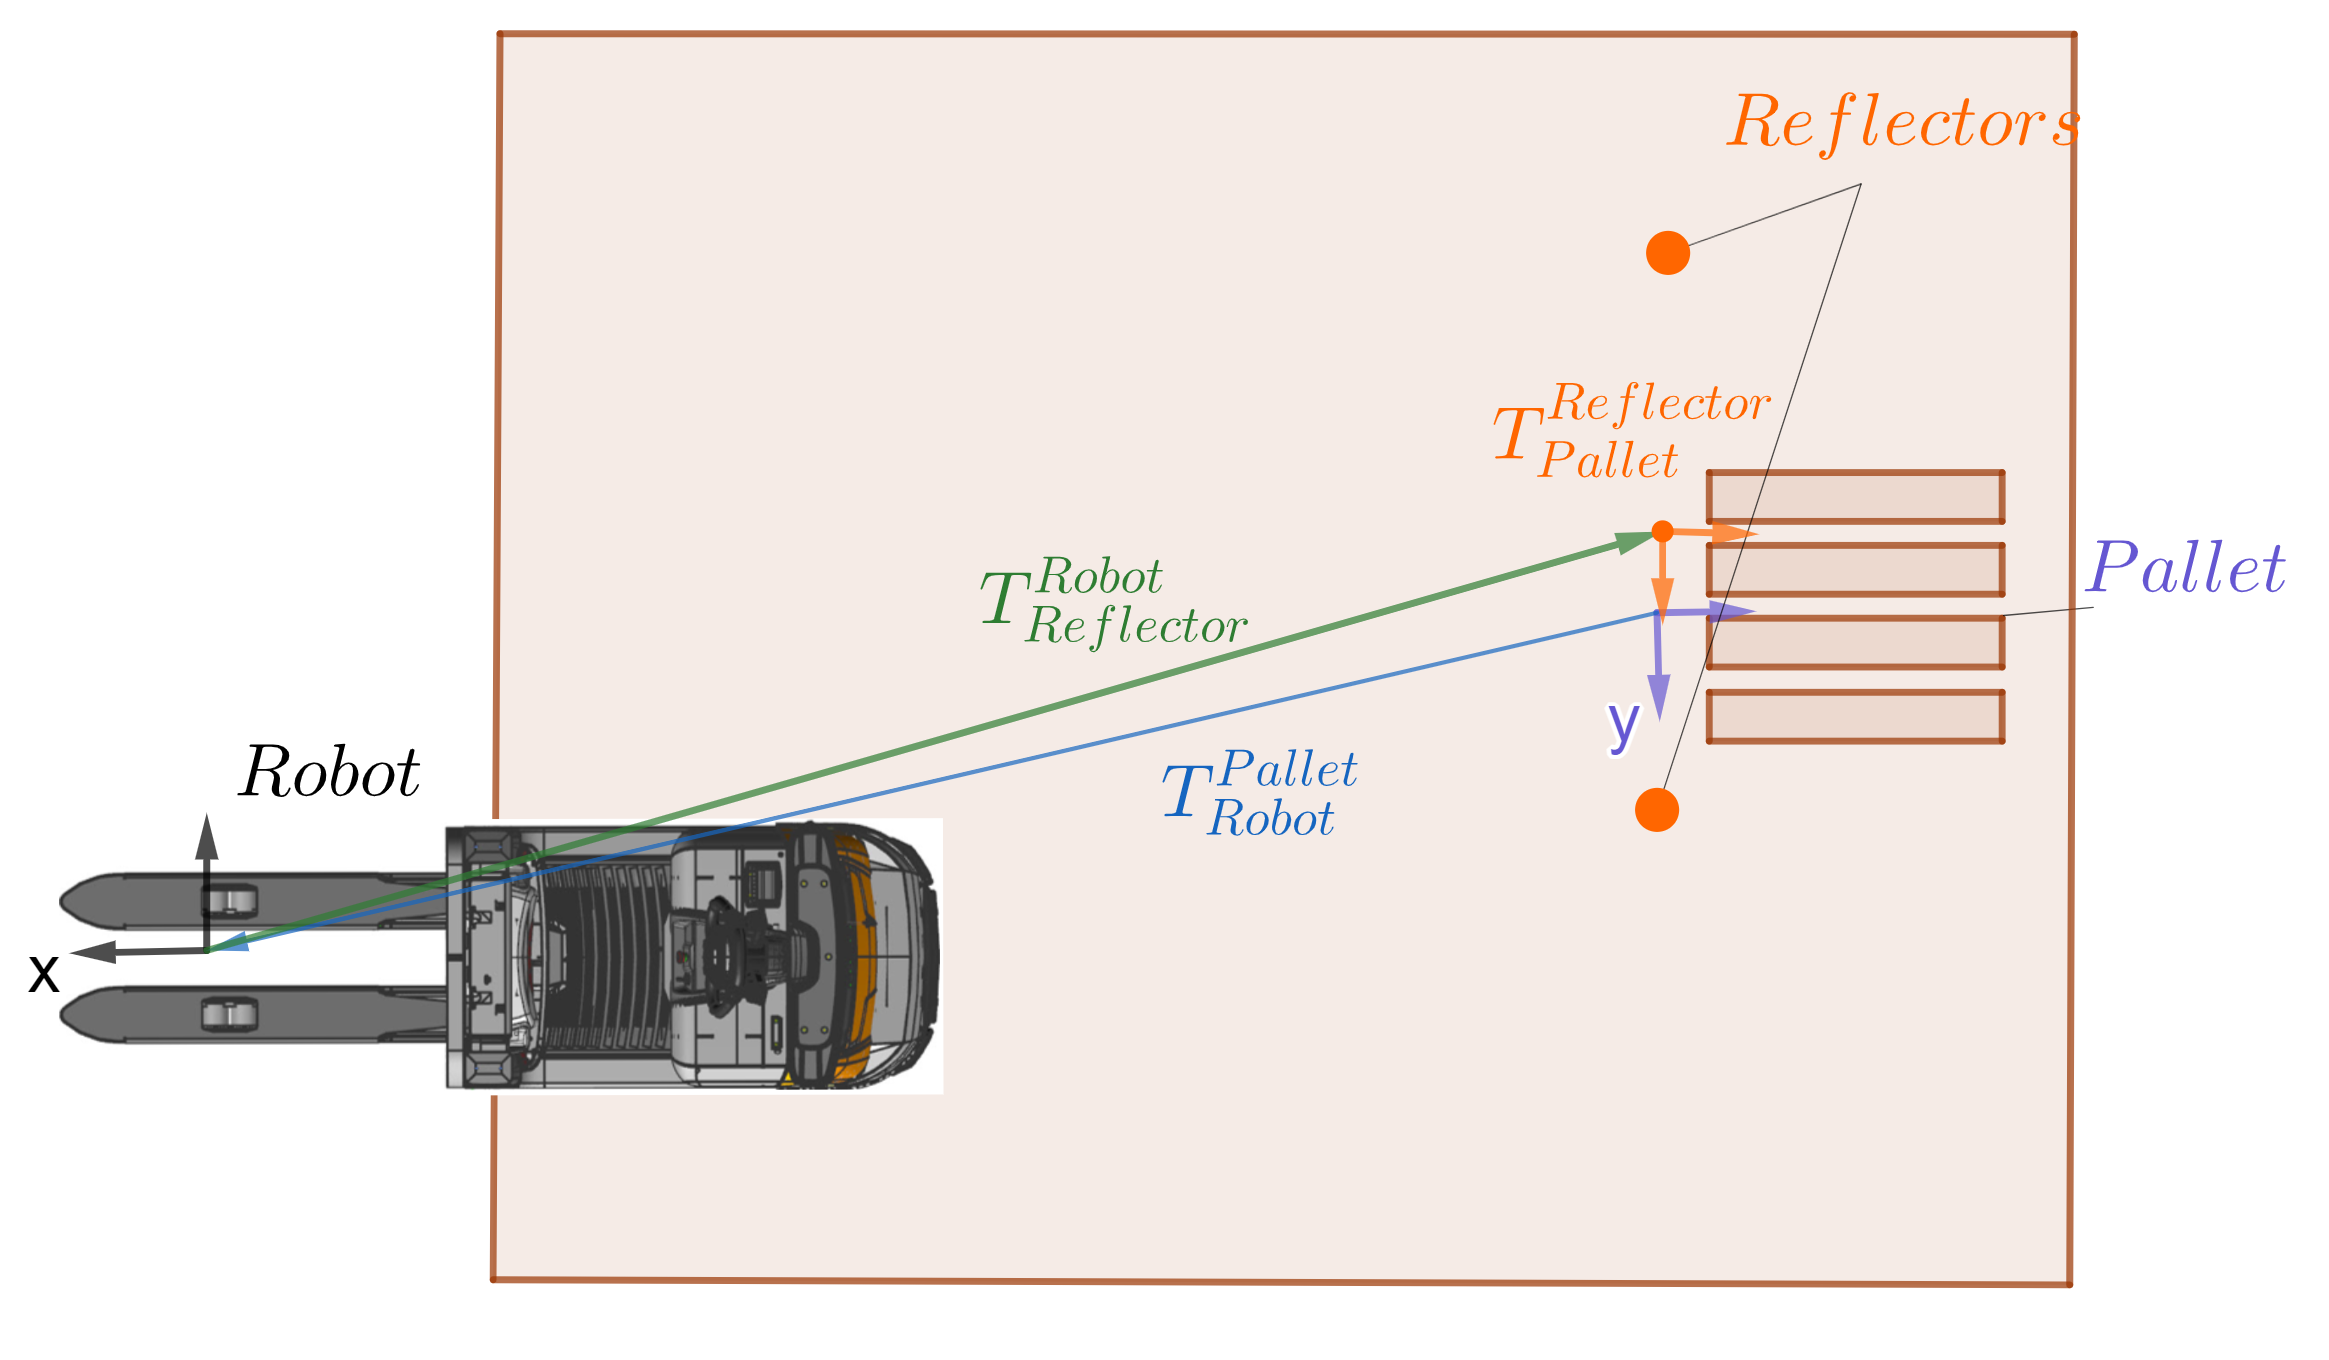
\includegraphics[width=4in]{images/Chap2/Transformation.png}\\
        \caption{Transformations From the Robot to the Pallet Frame Passing by the Reflector
        Frame}
        \label{Transformation}
        \end{center}    
\end{figure}
The transformations between the different objects are illustrated by figure \Ref{Transformation}.
\textbf{The Green Arrow} represents the Transformation from the Reflector to the Robot $T_{Reflector}^{Robot}$.
\textbf{The Orange Arrow} represents the Transformation from the Pallet to the Reflector $T_{Pallet}^{Reflector}$.
\textbf{The Blue Arrow} represents the Transformation from the Robot to the Pallet $T_{Robot}^{Pallet}$.

The general Pseudocode of the Path Generation is explained through Algorithm \Ref{alg:createSplines}.

\begin{algorithm}[H]
    \caption{Creation of a Spline by Points Interpolation}\label{alg:createSplines}

    \SetAlgoLined
    \KwData{points}
    \KwResult{createdNewSplineFromPoints}
    
    Initialize Spline\;
    
    SetInterrogationPoints(points)\;
    CreateCurveByInterpolation()\;
    
    max\_par $\gets$ Spline.GetMaxParameterVal()\;
    min\_par $\gets$ Spline.GetMinParameterVal()\;
    length $\gets$ Spline.GetFullCordLength()\;
    curvature\_change $\gets$ Spline.GetCurvatureChange()\;
    samples $\gets$ round(length / kSegmentLength)\;
    step $\gets$ (max\_par - min\_par) / samples\;
    
    \For{f $\gets$ min\_par + step \KwTo max\_par \textbf{by} step}{
        Spline.GetPosition(f, position)\;
        PathData.Spline.Position $\gets$ position\;
    }
    
    \Return{createdNewSplineFromPoints}\;
    
    \end{algorithm}




%TODO: check if section numbers are correct: ctrl+F section
\subsection{Path Evaluation}
Once the path has been created and the relevant information has been retrieved, the foundation is set to evaluate the 
quality of the generated paths. \textbf{The input for this section is a spline-based path pattern, and the 
output is a scalar value that reflects the quality of the path}.
Path evaluation allows to assess the quality of a path. From the vehicle's perspective, it enables the 
prediction of whether the path is mechanically and strategically feasible in terms of curves, sharp turns, direction 
changes, and other factors. This evaluation prevents the vehicle from following low-quality paths and paves the way 
towards optimization and selection of the best possible routes.
The literature proposes several approaches to path evaluation 
that have been tested and assessed in this work.

\subsubsection{Path Evaluation Techniques in Robotics}
 
When planning paths for robots in the Intralogistics or in any field in general, it is important to have the ability 
to quantify the quality of the resulting path. There exists different ways to judge the efficiency of the solution
and to which extent it accomodates the goal and optimizes the gaps that we are willing to improve.
This section studies the strategies that the literature followed while quantifying path quality in the robotics
field. It will look at the different indicators, why, and in which case they were used. 

\subsubsubsection{Core Metrics for Path Evaluation}
The key metrics that researchers focus on and try to improve can vary depending on the specific areas of 
optimization they are working on. For example, if the goal is to make a robot move faster, then time 
and speed might be the main metrics they study. On the other hand, if the focus is on making the robot 
navigate more safely, then the proximity to obstacles and collision avoidance would become the primary 
metrics. Therefore, the choice of metrics is closely linked to the particular goals that researchers 
aim to achieve in their optimization efforts.

According to Tang, S. H. et al. \cite{R20}, from 2011 to 2015, the second most common topic in the path 
planning research scope was path length. Path length is a key metric that helps us understand other 
important factors like travel time and energy consumption. By measuring the length of a path, we 
can get insights into how long it will take to travel and how much energy the robot might use. 
In other words, path length often reflects the overall efficiency and effectiveness of the route. 
Heiden, E et al. \cite{R23}, employed path length as one of the metrics used to evaluate the length of 
the paths generated by the algorithms they benchmarked. Their planners 
were configured to minimize path length, therefore, they measured the path lengths that were computed 
in 4 scenarios with applied to 17 path planners and 4 steering algorithms. They used path length,
along other metrics, to quantify the quality of paths after palnning and smoothing.
Besides, they compared the algorithms using the above-mentioned metrics in order to classify them
under the benchmark and to justify the choice of the best algorithm.  

In addition to path length, Path smoothness is crucial for robotics in general and especially 
in the intralogistics sector because it directly affects the efficiency and safety of robot 
operations. Smooth paths reduce the need for sudden stops or sharp turns, which helps robots 
maintain a steady speed and avoid unnecessary wear on their components. In intralogistics, 
where robots often work in busy environments with other machines and human workers, smooth 
paths also minimize the risk of accidents and product damage. Overall, ensuring path 
smoothness helps robots operate more reliably and effectively, leading to faster and 
more accurate material handling. Path smoothness reflects less cusps -sharp turns- and generally
less curvature which allows for smooth driving and smaller scale steering.
Curvature of a circle at a point \(x(t)\) is defined according to Gary D. Knott, in his book 
"Interpolating Cubic Splines" \cite{R34}, as the reciprocal of the radius at the same point as shown in
equation \Ref{kurv}.

\begin{equation}
    \kappa = \frac{1}{R}
    \label{kurv}
\end{equation}

For a cubic spline \( y = f(x) \), the curvature \( \kappa \) at a point \( x \) is given by:

\begin{equation}
\kappa = \frac{|f''(x)|}{\left(1 + \left(f'(x)\right)^2\right)^{3/2}}
\end{equation}

Heiden, E et al. \cite{R23}, also relied on curvature to determine path quality. They used it along 
path length and tracked it for the different scenarios and algorithms to measure their effectiveness.
Liu, S. et al. integrated path smoothness metric to quantify path quality for their benchmark to compare
motion planning algorithms\cite{R35}.
Although the above-mentioned sources used the metrics to evaluate their optimized solutions,
they did not mention the equations that they use to quantify those values.

Path clearance is another significant metric used to evaluate how well a robot can safely navigate 
its environment. It measures the distance between the robot's position along the path and any obstacles 
it might encounter. A larger path clearance means the robot has more space around it, reducing the risk 
of collisions and making the path safer. This metric is especially useful when optimizing paths, as it 
helps ensure that the robot can move smoothly without bumping into objects or other robots. 
Elshamli, A. et al. \cite{R17} have used path clearance as one of the indicators of path feasibility.
Clearance is measured as follows in \Ref{clear}:

\begin{equation}
    \sum_{i=1}^{n-2} \exp\left(a \cdot (g_i - \tau)\right)
    \label{clear}
\end{equation}

where \(g_i\) is the shortest distance from the \(i^{\text{th}}\) discrete position of the 
robot to the surrounding obstacles, and \(\tau\) is the desired clearance distance that 
guarantees safety. By focusing 
on path clearance, we can design routes that not only get the robot from one point to another efficiently 
but also do so in a way that minimizes risks and improves overall safety.

\subsubsubsection{Combinations of single metrics}

Some applications focus solely on minimizing path length. They use this single value as the 
metric for evaluating and distinguishing path solutions or for optimization. However, other 
applications require the combination of several metrics.
Elshamli, A. et al. \cite{R17} used a weighted sum of the Distance between two nodes, or two waypoints,
Path smoothness, and clearance as given by \Ref{evaluation}. 

\begin{equation}
    \text{eval}(p) = w_d \cdot \text{dist}(p) + w_s \cdot \text{smooth}(p) + w_c \cdot \text{clear}(p)
    \label{evaluation}
\end{equation}
The outcome of this evaluation function of each path is used as the fitness function for that path.
The fitness of each path serves later the evolution of the genetic algorithm.

Zhang B et al. \cite{R36}, deployed a nonlinear optimization problem that integrates path length and 
curvature variation over a spline-based path. The problem is constrained by the curvature limits, the 
parametrized location of the spline's control points, and the distance to obstacles.

Combining metrics for path evaluation should be done with a simple approach. Using more metrics can make 
the optimization process complex 
and slow, as the optimizer has to handle more variables. Using too many metrics can lead to overfitting, 
where the model becomes overly sensitive to specific parameters and may not generalize well to new data. 
This can result in inconsistent results that may favor or neglect certain parameters in different situations.. 
By keeping the metrics to a 
manageable number, we ensure that the optimization remains efficient and the impact of each metric 
is clear and easy to interpret. 
Using a more metrics like computational time, number of cusps or direction changes, solvability percentage
or predicted speed or travel time can be efficient for evaluating path planning algorithms and benchmarking some
usecases as in \cite{R23}.


\subsubsection{Implementation of Path Evaluation Techniques}
By analyzing the spline,  key characteristics of the path can be determined, such as its length, curvature, and 
the time required to traverse it. The following requirements are essential for developing a robust path 
evaluation formula:
\begin{itemize}
    \item The formula used to evaluate the path must be \textbf{simple} enough to be easily integrated into an optimization process.
    During path planning, optimization algorithms are often employed to find the best possible path according to certain 
    criteria. These algorithms require objective functions that can be computed efficiently. A complex or computationally 
    expensive formula may slow down the optimization process or make it impractical for real-time applications. 
    Therefore, the path evaluation formula should be simple, allowing for quick calculations that can be repeatedly 
    applied within an optimization loop. This simplicity also facilitates its integration with existing optimization 
    frameworks.
    \item The formula should include a \textbf{normalization} step to ensure that different paths can be compared on a common scale.
    Paths can vary significantly in terms of length, curvature, and other characteristics. To make meaningful 
    comparisons between paths, it’s essential to normalize these metrics. Normalization involves scaling the values of 
    each metric (e.g., path length, curvature change) relative to a reference value, such as the characteristics of 
    a potential ideal path. By normalizing the path metrics, it is ensured that the evaluation formula is 
    dimensionless and that the different aspects of the path (e.g., length versus curvature) are balanced 
    appropriately. This step is crucial when combining multiple metrics into a single evaluation score, as it 
    prevents any one metric from disproportionately influencing the final result.
    \item The evaluation should \textbf{prioritize paths that minimize length and curvature}.  In most path planning scenarios, 
    especially for vehicles or robots, the goal is to find the most efficient path from point A to point B. 
    Efficiency can be measured in terms of:
    \begin{itemize}
        \item Path Length: Shorter paths are generally preferred because they reduce the distance the vehicle or robot 
        needs to travel, therefore saving energy and time.
        \item Curvature: Paths with less curvature are preferred because sharp turns can be difficult for vehicles 
        to navigate, especially at higher speeds. Minimizing curvature reduces the risk of instability of the vehicle.
    \end{itemize}
    
\end{itemize}

The combination of these requirements leads to a path evaluation formula that is both practical and effective. 

To implement this path evaluation effectively, it was essential to accurately measure the path's length and curvature 
change, as these are critical components of the evaluation formula. 

The path length was calculated by summing the distances between consecutive points along the spline, ensuring that 
even small variations in the path's trajectory were captured as given by equation \Ref{length_formula}.
\begin{equation}
    L = \sum_{i=\min \ \text{par}}^{\max \ \text{par}} s(i)
    \label{length_formula}
\end{equation}
where \( s(i) \) denotes the length of the \(i\)-th curve segment of the spline measured between two points of the 
spline using Euclidean distance.

The curvature change of a spline path is quantified by evaluating how the curvature of the path varies along its Length.
The curvature change (\( cc \)) calculated by:

\begin{equation}
cc = \int \frac{d(k)}{d(s)} \, ds
\end{equation}

represents the total variation in curvature along the path, where \( \frac{d(k)}{d(s)} \) measures how curvature itself 
changes as a function of arc length, and integrating this derivative over the path provides a comprehensive metric of 
curvature variation.

As this equation involves an integral, it has to be approximated in order to compute it in a programming environment.
The approximation is conducted through a discretization of the path into a series of small segments. For each segment, 
the curvature change and segment length are approximated. Let \( \Delta s(i) \) denote the length of the \(i\)-th segment 
and \( \Delta k(i) \) the change in curvature over this segment.
Then, the trapezoidal rule is used to approximate the integral. 
This is achieved by summing up the ratio of curvature change to segment length over all segments as given by 
equation \Ref{curvature_change}:
\begin{equation}
cc = \sum_{i = \min \ \text{par} + \text{step}}^{\max \ \text{par}} \frac{\Delta k(i)}{\Delta s(i)}
\label{curvature_change}
\end{equation}

Mathematically, if \(k(i)\) is the curvature at the \(i\)-th segment, then \( \Delta k(i) \) can be expressed as:
\begin{equation}
    \Delta k(i) = \left| k(i) - k(i-1) \right|
\end{equation}
where \(k(i-1)\) is the curvature of the previous segment. The absolute value is used to prevent cancellation of terms:
curvature can be negative or positive according to the convexity or concavity of the curve. When summed together,
a neutralization could happen resulting in an insignificant value. This could be solved by introducing the squarred 
difference between \(k(i)\) and \(k(i-1)\). However, it will minimize the result to a negligible value for the 
overall analysis as the curvature values are around the magnitude of \(10^{-2}\) or less.

The summation provides a cumulative measure of curvature changes relative to the segment lengths along the entire path, 
offering insight into the overall curvature dynamics of the spline. The formula for \(cc\) evaluates the total effect 
of curvature changes normalized by segment lengths over 
the path. This metric is useful for understanding how the path’s curvature varies and helps in optimizing paths 
to ensure smooth and efficient navigation.

To develop a cost function that integrates both path length and curvature, we explore two distinct approaches: 
Exponential Weighted Path Evaluation and Normalized Weighted Path Evaluation. These approaches use weights to 
prioritize the significance of each component in the evaluation process. 

\subsubsubsection{First approach: Exponential Weighted Path Evaluation}
The Exponential Path Evaluation is based on A. Elshamli, et al. method \cite{R17}. As explained in section 2.3,
they consider path length, smoothness and clearance combined in a weighted cost function.
Their approach of measuring path length and smoothness is considered here with some changes to fit it into the use case.

Path length term is measured in \cite{R17} as follows:
\begin{equation}
d = \sum_{i=1}^{n-1} d(s_i)
\end{equation}

Whereas, Path smoothness is measured as follows:

\begin{equation}
d = \sum_{i=2}^{n-1} \exp(a(\theta_i - \alpha))
\end{equation}

where \( \theta_i \) represent the steering angle at the \(i\)-th segment, and \( \alpha \) denote the desired 
steering angle.

Besides path clearance, those values are weighted and summed.
This summation is not normalized given that it adds the distance term which has a unit to the smoothness and 
clearance terms that are exponential functions results. 
In this approach of the work, the exponential function is used for normalization of distance and curvature change 
terms. The length term is given by:
\begin{equation}
    \text{Length Term} = e^{\beta \cdot \left(\text{current}_L - \text{ref}_L\right)}
    \end{equation}
    
    \noindent
    The curvature change term is given by:
    \noindent
    
    \begin{equation}
    \text{Curvature Change Term} = e^{\alpha \cdot \left(\text{current}_{cc} - \text{ref}_{cc}\right)}
    \end{equation}
    
    \noindent
    where: 
    \newline
    - \textit{current} refers to the path being evaluated and \textit{ref} refers to the reference path.
    \newline
    - \(\alpha\) and \(\beta\) are factors that rationalize the exponential terms because the length is in the range 
    of thousands of millimeters while the curvature is around the magnitude of \(10^{-3}\).
    Without these factors, the two terms would differ significantly, leading to incorrect analysis of the impact of each term.
    
\noindent The cost function of the weighted terms is given by equation \Ref{exp_function}:

\begin{equation}
Z^{\ast }=\arg \min \left(\omega_{c} \cdot e^{\alpha \cdot \left( \text{current}_{cc} - \text{ref}_{cc} \right)} + \omega_{L} 
\cdot e^{\beta \cdot \left( \text{current}_L - \text{ref}_L \right)} \right)
\label{exp_function}
\end{equation}
\noindent
with constraints: \[K(i)\ <\ K_{\max}\]
\noindent

and \[\text{RobotFootprint}(\mathbf{p}_i) = 0 \quad \text{for all } i\]


where \begin{itemize}
    \item \(\omega_c\) and \(\omega_L\) are the weights assigned to the curvature change term and the length term, 
    respectively. These weights determine the relative importance of curvature change and path length in the overall 
    evaluation. 
    \item \(\ K_{\max}\) the maximum tolerated curvature
    \item \( \mathbf{p}_i \) represent the \( i \)-th scan point in space. 

    \item \( \text{RobotFootprint}(\mathbf{p}_i) \) be a boolean function that returns 1 if the point \( \mathbf{p}_i \) 
    lies within the robot's footprint (polygon) and 0 otherwise.
    
\end{itemize}


\subsubsubsection{Second approach: Normalized Weighted Path Evaluation}

The Normalized Weighted Path Evaluation is based on the division of the path's Length
and Curvature Change measured respectively using the equations \Ref{Length_formula} and 
\Ref{curvature_change} respectively by the reference path's Length and Curvature Change. 
The length term is given by:
\begin{equation}
    \text{Length Term} = \frac{\sum_{i=\min \text{ par}}^{\max \text{ par}} s(i)_j}{\sum_{i=\min \text{ par}}^{\max \text{ par}} s(i)_{\text{ref}}}
\end{equation}

\noindent
The curvature change term is given by:

\begin{equation}
    \text{Curvature Change Term} = \frac{\sum_{i=j \min \text{ par}}^{j \max \text{ par}} \frac{\Delta k(i)_j}{\Delta s(i)_j}}{\sum_{i=\text{ref} \min \text{ par}}^{\text{ref} \max \text{ par}} \frac{\Delta k(i)_{\text{ref}}}{\Delta s(i)_{\text{ref}}}}
\end{equation}

where \( j \) denotes the current path being evaluated.

\noindent The cost function of the weighted terms is given by equation \Ref{Norm_function}:
\begin{equation}
    Z^{\ast} = \arg \min \left( \omega_C \cdot \frac{\sum_{i=\text{j min par}}^{\text{j max par}} \frac{\Delta k(i)_j}
    {\Delta s(i)_j}}{\sum_{i=\text{ref min par}}^{\text{ref max par}} \frac{\Delta k(i)_{\text{ref}}}
    {\Delta s(i)_{\text{ref}}} } + \omega_L \cdot \frac{\sum_{i=\text{min par}}^{\text{max par}} s(i)_j}
    {\sum_{i=\text{min par}}^{\text{max par}} s(i)_{\text{ref}}} \right)
\label{Norm_function}
\end{equation}

\noindent
with constraints: \[K(i)\ <\ K_{\max}\]
\noindent

and \[\text{RobotFootprint}(\mathbf{p}_i) = 0 \quad \text{for all } i\]


where \begin{itemize}
    \item \(\omega_c\) and \(\omega_L\) are the weights assigned to the curvature change term and the length term, 
    respectively. These weights determine the relative importance of curvature change and path length in the overall 
    evaluation. 
    \item \(\ K_{\max}\) the maximum tolerated curvature
    \item \( \mathbf{p}_i \) represent the \( i \)-th scan point in space. 

    \item \( \text{RobotFootprint}(\mathbf{p}_i) \) be a boolean function that returns 1 if the point \( \mathbf{p}_i \) 
    lies within the robot's footprint (polygon) and 0 otherwise.
    
\end{itemize}

The algorithm that measures the path quality is detailed through Pseudo Code \Ref{EvaluationAlgorithm}.

\begin{algorithm}[H]
    \caption{Path Evaluation Algorithm}\label{EvaluationAlgorithm}

    \SetAlgoLined
    \KwData{Spline Path, set of scan points $P$}
    \KwResult{Evaluation result}
    
    Initialize Metric\;
    
    \If{local\_max\_curvature > maximum\_curvature\_}{
        metric.curvature\_change\_ $\gets$ curvature\_KnockOut\_factor $\cdot$ local\_curv\_change\;
    }
    \Else{
        metric.curvature\_change\_ $\gets$ local\_curv\_change\;
    }
    
    metric.length\_ $\gets$ metric.calculate\_length\_metric(gen)\;
    
    \For{each point $p_i$ in $P$}{
        test $\gets$ RobotFootprint($p_i$)\;
        
        \If{test == 0}{
            result $\gets$ obstacle\_KnockOut\;
        }
        \Else{
            result $\gets$ EvaluationFunction(curvature, length)\;
        }
    }
    
    \Return{result}\;
\end{algorithm}

\newpage
\subsection{Path Optimization}
After successfully developing the tools to partition the stations, create spline-based pattern paths, and evaluate their quality 
in line with the trucks' properties and target outcomes, the paths are ready for the optimization phase.
\textbf{The input of this section is a range of paths along with their evaluation scores and the output is the optimal 
path to be driven.}

\subsubsection{Utility}
The utility of the path optimization process lies in its ability to identify the most efficient and effective path for the 
vehicle to follow, based on various criteria. By considering key factors such as path length, curvature, and smoothness, 
the optimization algorithm ensures that the selected path not only adheres to the vehicle's operational constraints but 
also minimizes risks associated with challenging maneuvers. This process plays a crucial role in improving overall system 
performance, as it helps reduce fuel consumption, wear on vehicle components, and driving complexity. Additionally, 
the optimized path leads to better time efficiency and safer operations, particularly in complex environments where 
tight turns or narrow spaces can hinder navigation.

\subsubsection{Implementation}
As discussed in section 3.1, The meta-heuristic approach is used to optimize the spline-based pattern paths. 
Based on the Literature review the choice was made around testing 5 meta-heuristic optimization algorithms then 
assessing each algorithm's performance. The algorithms are: Particle Swarm Optimization (PSO), Differential Evolution (DE),
Genetic Algorithms (GA), Simulated Annealing (SA), and Ant Colony Optimization (ACO). Those algorithms were selected due 
to their capabilities of solving the local optima problematic and their applications in robotics path planning although 
considered recent for some of the algorithms. 

The optimization process is detailed through Algorithm \Ref{optimization}. After initializing the optimization problem-related
parameters, The algorithm starts the evolution of the generations or the iterations. In each iteration it generates a fixed 
number of individuals. \textbf{The decision vector of each individual is the transition point. The optimization algorithm
starts by placing random transition points inside the subpolygons}. First the initial individuals are generated. 
For Population based algorithms like GA and DE, generate an initial population of candidate points $(x, y)$, for swarm-based algorithms
like ACO and PSO, 
initialize particles or ants randomly, For Simulated Annealing (SA), start with a single solution point $(x, y)$.\\
Each transition point is used to generate a path as explained
in section 3.3.2 then evaluated through the method in section 3.3.3. The evaluation result is the fitness of the path that the 
optimization algorithm bases its results on. By now the initial generation is completed. Then, the algorithm iterates until 
the maximum number of iterations is met. The reason behind choosing a maximum number of iterations is that the fitness function 
is not tangible. It can vary according to many factors like station configuration and dimensions and navigation environments.
Tuning a goal fitness that fits all cases can be limiting if it set higher than the possible optimal fitness and causes sinking in 
suboptimal solutions or can constrain the optimizer if set too low: the optimizer can quit without solutions.
Then the algorithm proceeds to generate new points following the meta-heuristic algorithm:

\begin{itemize}
    \item GA: Apply selection, crossover, and mutation to generate new points $(x, y)$.
    \item DE: Create new trial points by combining the difference between vectors of points.
    \item PSO: Update positions of particles based on their velocities, influenced by the personal and global best.
    \item SA: Randomly perturb the current point $(x, y)$ and generate a new path.
    \item ACO: Ants select the next points $(x, y)$ based on pheromone trails and heuristic information.
\end{itemize}
Afterwards, it generates Corresponding Paths, evaluates Fitness of New Paths and updates the Population or Solution Set
in relevance to the meta-heuristic algorithm: 
\begin{itemize}
    \item GA: Select the next generation of points based on fitness, using techniques like elitism or tournament selection.
    \item DE: Retain points with better fitness, replacing weaker ones.
    \item PSO: Update the personal best positions and global best positions of particles.
    \item SA: Accept or reject new points based on a probabilistic function that includes temperature.
    \item ACO: Update pheromone trails based on the quality of the paths found, and reduce pheromone levels globally (evaporation).
\end{itemize}
The last step of each iteration is to update the algorithm parameters:
\begin{itemize}
    \item GA/DE/PSO: Adjust crossover rates, mutation rates, or particle velocities.
    \item SA: Reduce temperature according to the cooling schedule to reduce acceptance of worse solutions over time.
    \item ACO: Evaporate pheromone globally and reinforce the best paths with additional pheromone.
\end{itemize}
Once the stopping criteria is met, the algorithm returns the best path that it found.

This Algorithm is ran once for each of the subpolygons. The optimization happens for both subpolygons, each 
optimizer returns an optimal path that uses the corresponding subpolygon.
Then, the results from both optimizers are compared and the fittest is considered as the overall
fittest path. 

For the application of these algorithms, Pagmo library was used. Pagmo is an open-source scientific library designed for 
C++ that specializes in optimizing massively parallel problems. It was developed between the Max Planck Institute for 
Astronomy and the Advanced Concepts Team, at the European Space Research and Technology Center \cite{R45}.
Pagmo provides an exhaustive toolset of meta-heuristic optimization techniques including the original Algorithms
and the improved versions. 

\subsubsubsection{Obstacle Avoidance in the Pattern Based Approach}
This approach is designed for complex, dynamic environments characterized by an abundance of obstacles, such 
as Operators, Pallets, Materials, Shelves, and other vehicles, both inside and outside the station perimeter. 
To navigate these environments, an obstacle avoidance feature is essential. The obstacle avoidance mechanism, 
integrated into the Pattern-Based Solution, is managed by the Optimizer, which assigns high penalties 
(referred to as "Knockout" values) to paths that collide with or come too close to obstacles 
(Fitness values $\lll$ Knockout). This approach, as detailed in Algorithm \Ref{EvaluationAlgorithm}, 
effectively eliminates colliding paths by making them unfavorable during optimization. For instance, 
as shown in Figure \Ref{Obstacle}, when obstacles block one of the subpolygons of the station, the 
Optimizer selects an alternate subpolygon. However, this method has limitations—if both subpolygons 
are blocked, the pattern cannot navigate around the obstacles. To address this, two additional 
waypoints are introduced: one between the robot and the transition point, and the other between 
the transition point and the destination. These waypoints increase flexibility by allowing the path 
to deviate from nearby obstacles. Their positions are optimized along with the transition points, as 
illustrated in Figure \Ref{Add_waypoints}, ensuring that each path candidate is created and evaluated 
using the same Evaluation approach.


\begin{figure}[H]
    \begin{center}
        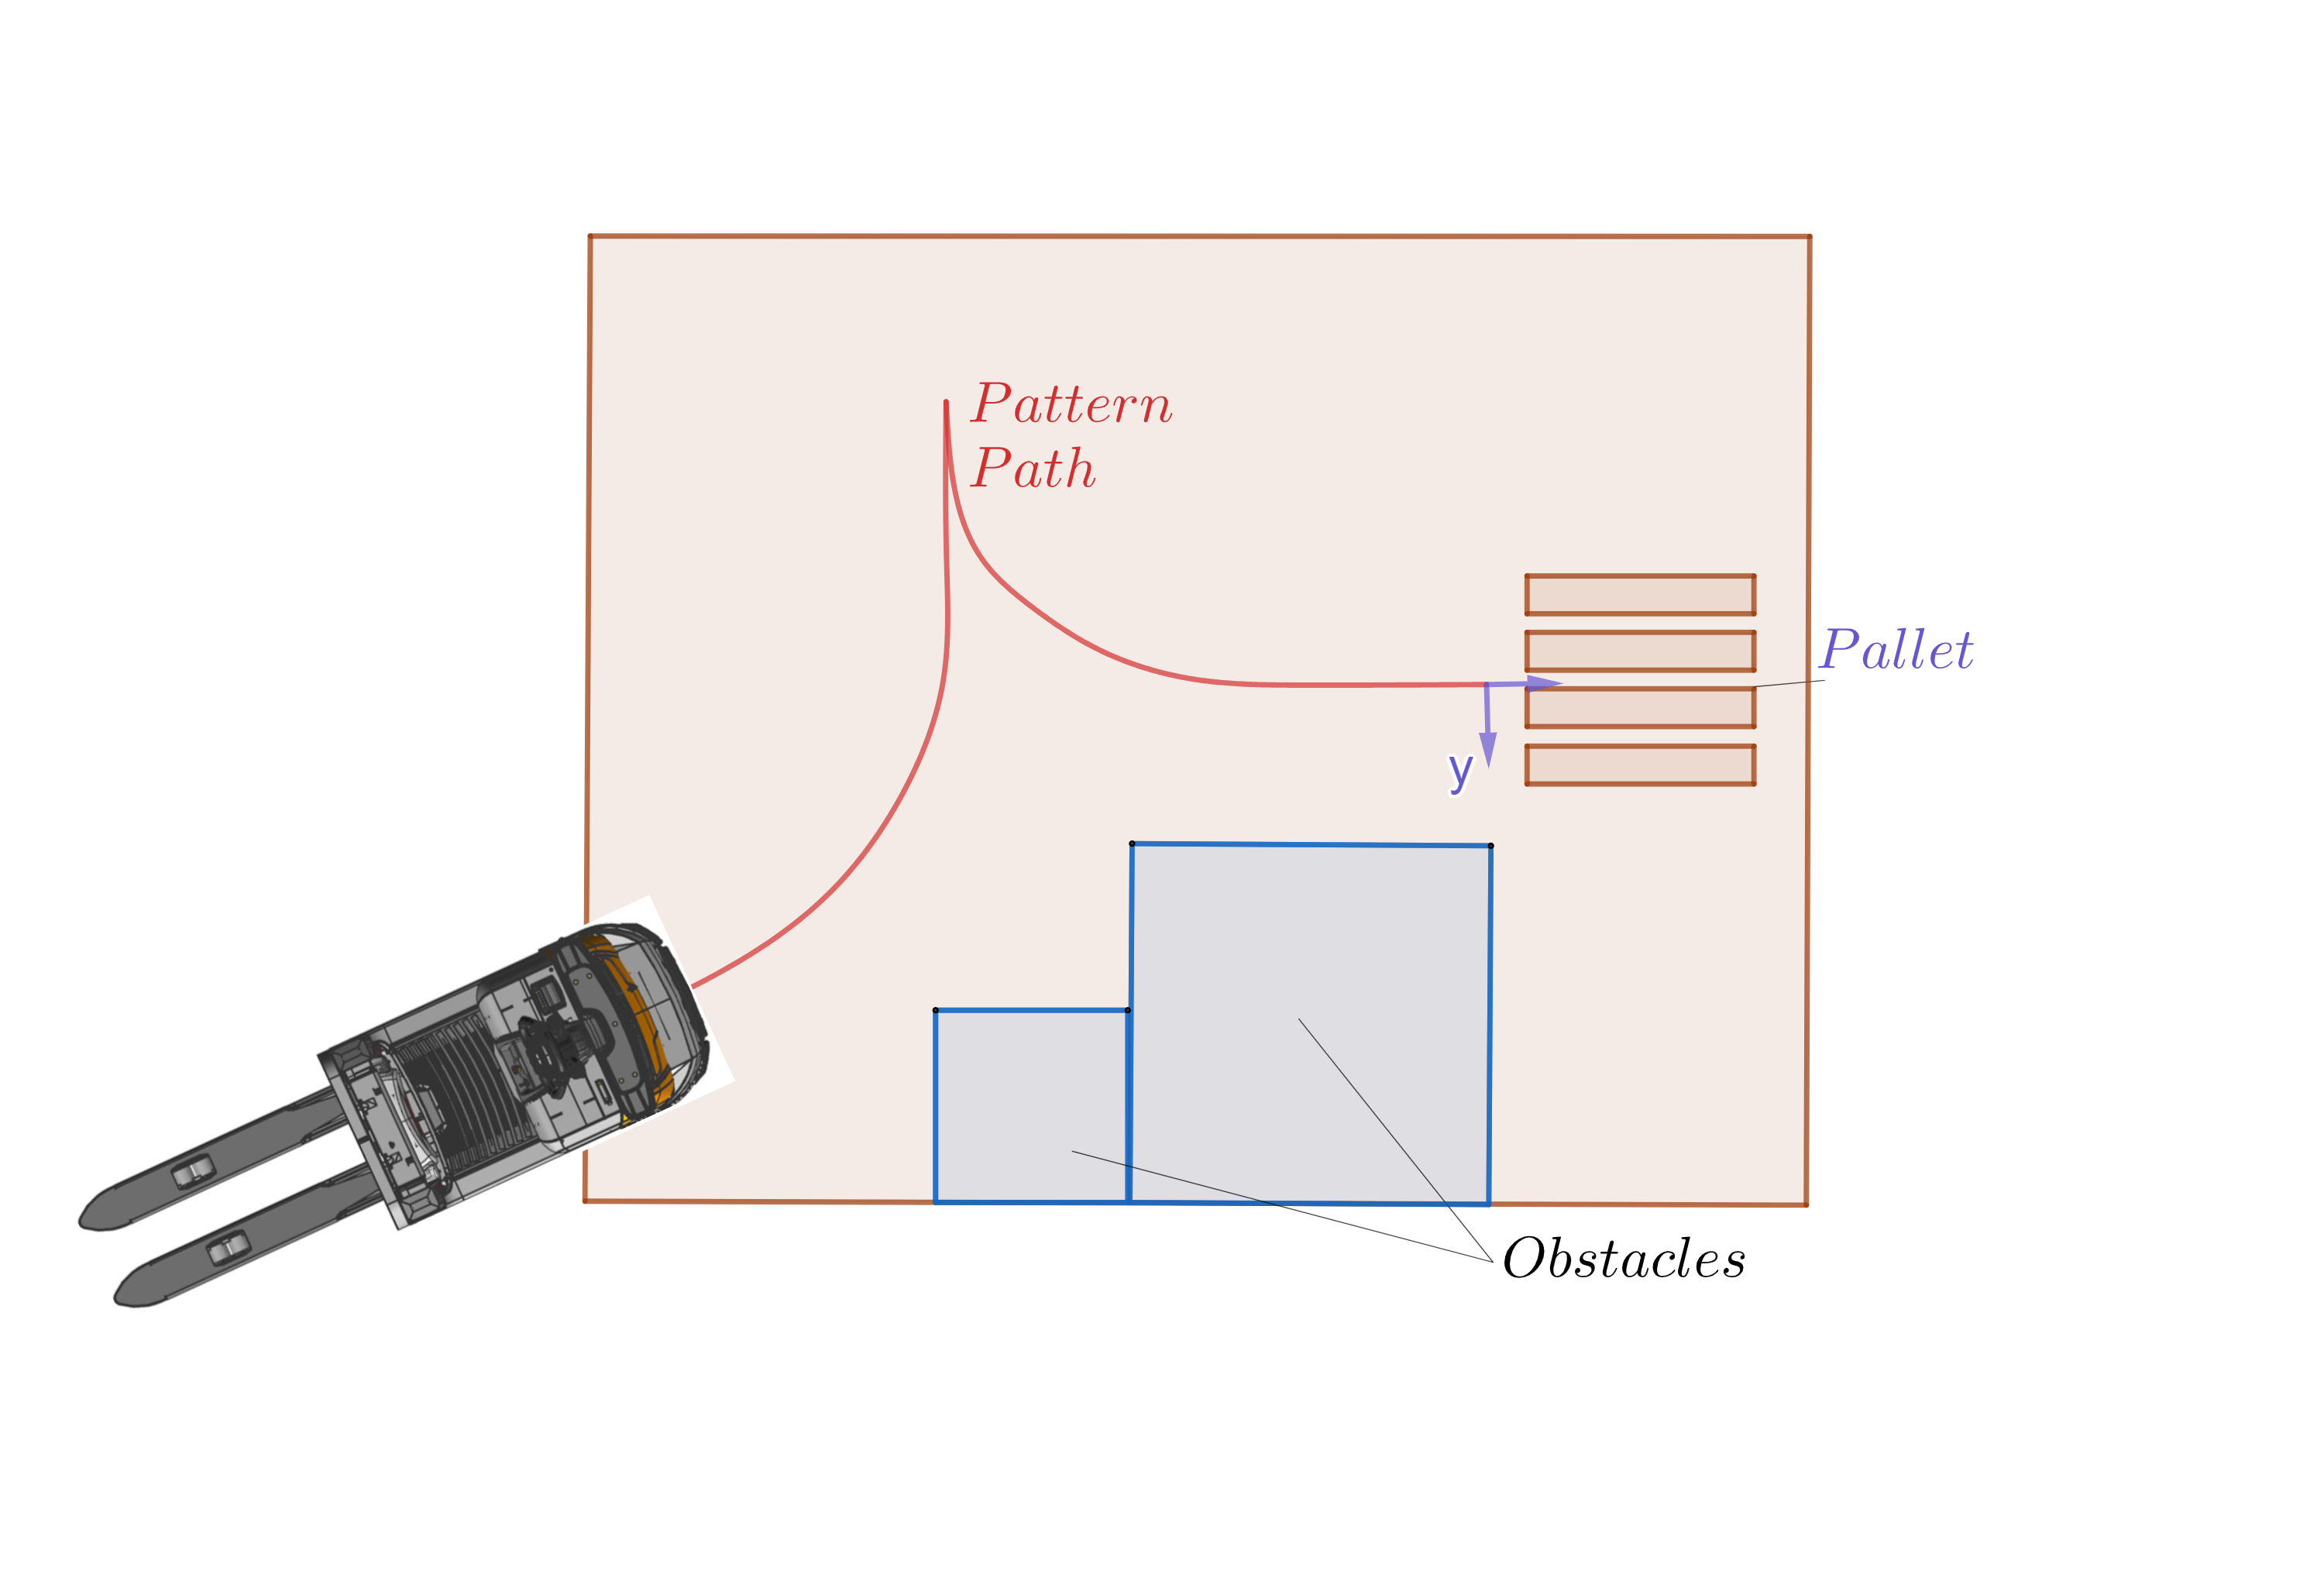
\includegraphics[width=5in]{images/Chap2/Obstacles_In_Station.png} % Replace with your figure
        \caption{Simulated Environment of the Station With Obstacles Blocking a Transition side}
        \label{Obstacle}
        \end{center}    
\end{figure}


\begin{figure}[H]
    \begin{center}
        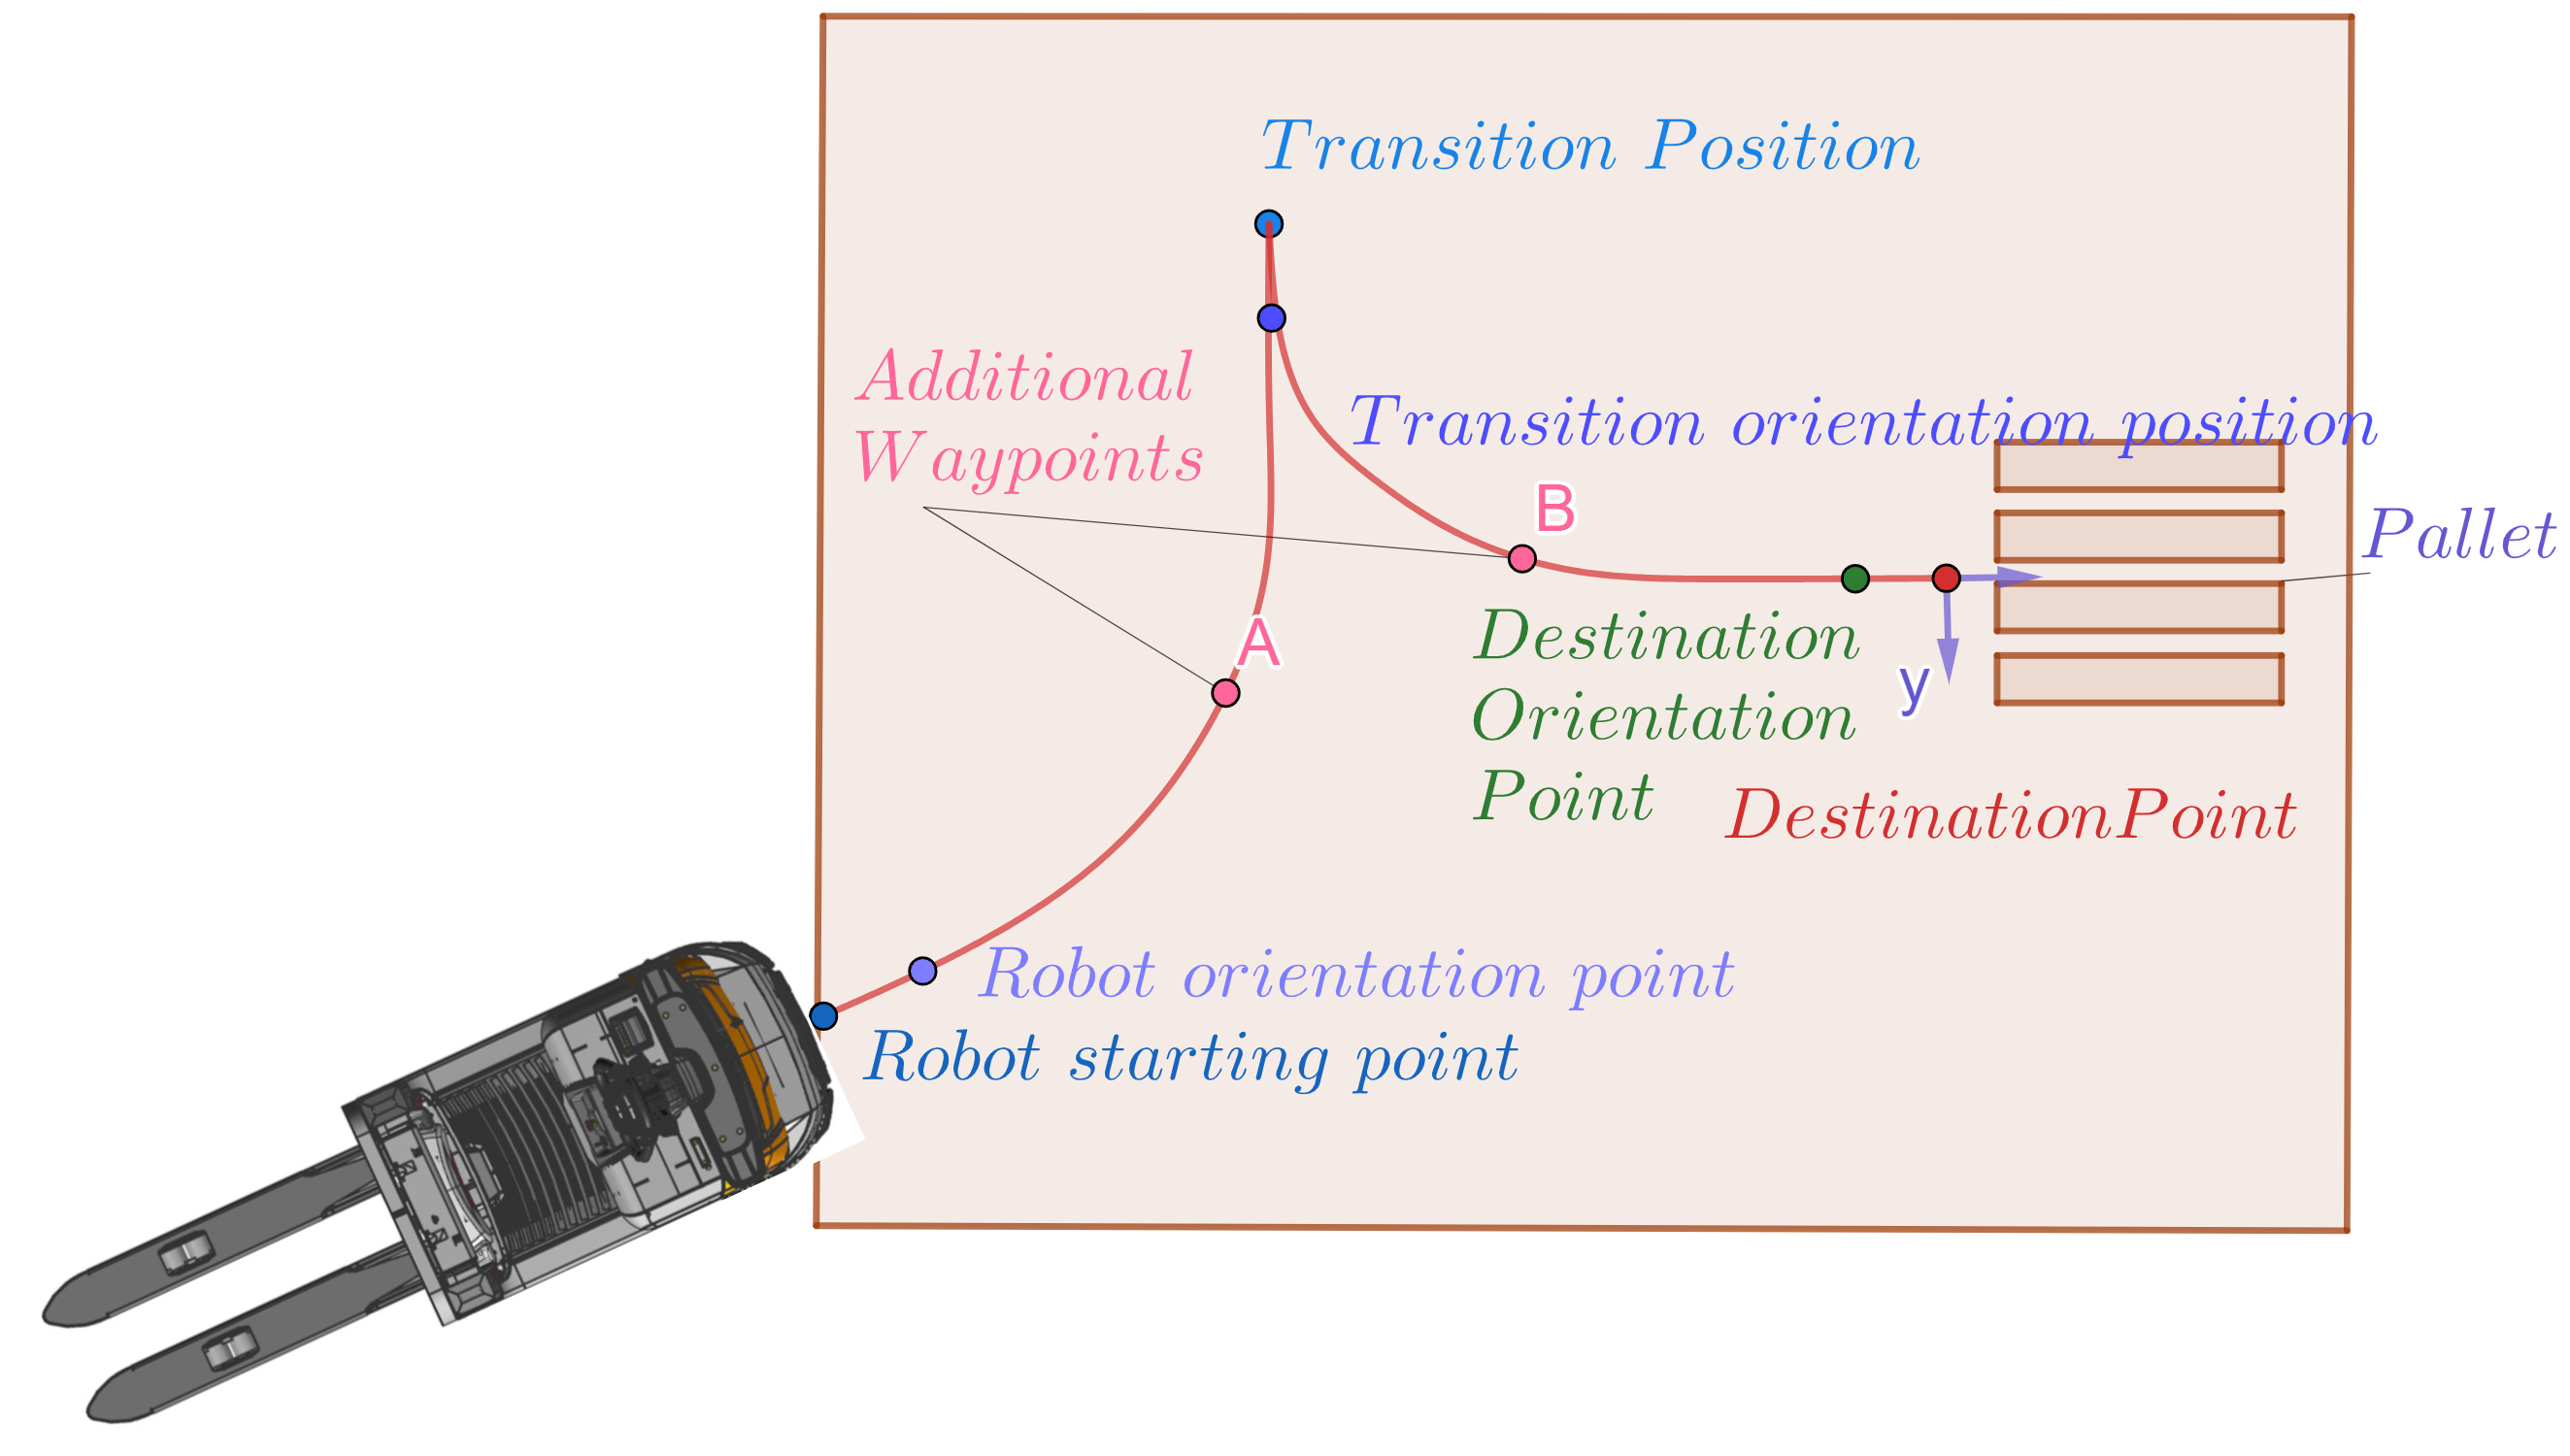
\includegraphics[width=4.5in]{images/Chap2/Add_waypoints.png} % Replace with your figure
        \caption{Simulated Environment of the Station with the added waypoints to enhance obstacle avoidance}
        \label{Add_waypoints}
        \end{center}    
\end{figure}


\begin{algorithm}[H]
    \caption{Generic Optimization Algorithm with Path Evaluation}\label{optimization}
    \KwIn{Problem parameters, Population size, Max iterations, Algorithm-specific parameters}
    \KwOut{GeneratedOptimalPath}
    
    \SetKwBlock{Begin}{begin}{end}
    
    Initialize  
    population size, max iterations,algorithm-specific parameters;\\
    \textbf{Initialize Population of Points}\\
    Generate an initial population of candidate points $(x, y)$.\\

    \textbf{Evaluate Fitness for Initial Paths}\\
    CreateEvaluationPath$(x, y)$;\\
    MeasureNormalizedMetric(path);    
    \textbf{Repeat until Termination Condition Met (max iterations ):}\\
    \Begin{
        Generate New Points\\
        Generate Corresponding Paths\\
        Evaluate Fitness of New Paths\\
        Update Population or Solution Set\\

        \textbf{Algorithm-Specific Update Step}\\
    }
    
    \textbf{Return Best Point and its Path:}\\
    Return the best point $(x, y)$ and its corresponding path found during the search process.
    \end{algorithm}

    

\section*{Conclusion}

This chapter focused on the development and implementation of the optimized local path planning 
approach. The geometric partitioning of the station allows the robot to identify zones where path 
transitions can be made. Paths were generated using spline theory and evaluated with a cost function 
based on path length and curvature change. Path optimization was subsequently applied to minimize the cost 
function value, ensuring effective navigation within the warehouse. With the development phase complete, 
the next step is to test and validate the proposed solution in practical scenarios.